%*************************************
% บทที่ 4
%*************************************
\chapterTitle{4}{ผลการดำเนินงาน}

\hspace*{1.3em}
ในการพัฒนาระบบแพลตฟอร์มคลาวด์เพื่อสนับสนุนกิจกรรมการเรียนการสอนและงานวิชาการ ได้ดำเนินการออกแบบและพัฒนาระบบที่ประกอบด้วย 3 บริการซอฟต์แวร์หลัก คือ ส่วนติดต่อผู้ใช้ (Frontend) ส่วนบริการ API (API Service) และส่วนประมวลผลงานจัดการเครื่องเสมือน (VM Operations Service) ร่วมกับบริการสนับสนุนสำหรับการยืนยันตัวตน ฐานข้อมูล ระบบคิวงาน พื้นที่จัดเก็บไฟล์ และระบบติดตามการทำงาน
ในบทนี้จึงนำเสนอผลการดำเนินงานในมุมของโครงสร้างรีโพซิทอรี องค์ประกอบของแต่ละบริการ เทคโนโลยีที่ใช้ เอกสารประกอบการใช้งาน และตัวอย่างหน้าจอของระบบที่พัฒนาขึ้นจริง โดยยึดตามสภาพแวดล้อมของโค้ดปัจจุบันซึ่งแยกเป็นหลายรีโพซิทอรีและติดตั้งใช้งานร่วมกันในลักษณะ Microservices Architecture
\section{โครงสร้างโครงงานหลัก}
\hspace*{1.3em}
จากการออกแบบและพัฒนาระบบแพลตฟอร์มคลาวด์เพื่อสนับสนุนกิจกรรมการเรียนการสอนและงานวิชาการ โครงงานฉบับปัจจุบันไม่ได้จัดเก็บแบบ Monorepo แต่แบ่งออกเป็น 4 รีโพซิทอรีหลักที่ทำงานร่วมกัน ได้แก่ \textbf{Midori}, \textbf{Momoi}, \textbf{Yuzu} และ \textbf{Yuuka} เพื่อให้สามารถพัฒนา ทดสอบ และติดตั้งใช้งานแต่ละส่วนได้อย่างเป็นอิสระ

\subsection{รีโพซิทอรี Midori}
\hspace*{1.3em}
รีโพซิทอรี \textbf{Midori} เป็นส่วนติดต่อผู้ใช้ของระบบ พัฒนาด้วย Next.js และ React ทำหน้าที่นำเสนอหน้าเว็บสำหรับนักศึกษา อาจารย์ และผู้ดูแลระบบ ภายในรีโพซิทอรีนี้มีโครงสร้างสำคัญ เช่นโฟลเดอร์ src/app สำหรับหน้าและ route หลักของระบบ, src/components สำหรับองค์ประกอบส่วนติดต่อผู้ใช้, src/hooks และ src/lib สำหรับตรรกะร่วม, รวมถึงไฟล์กำหนดค่าอย่าง package.json, next.config.ts และ components.json
\begin{mycustomenum2}
    \item \textbf{Landing Page และ Login Flow} สำหรับการเข้าถึงระบบและเข้าสู่กระบวนการยืนยันตัวตน
    \item \textbf{Dashboard ตามบทบาทผู้ใช้} สำหรับนักศึกษา อาจารย์ และผู้ดูแลระบบ
    \item \textbf{Client สำหรับเรียก API} ที่เชื่อมต่อกับ Momoi และบริการยืนยันตัวตนผ่าน OpenAPI
\end{mycustomenum2}
\hspace*{1.3em}
การแยกส่วนติดต่อผู้ใช้ออกมาเป็นรีโพซิทอรีเฉพาะช่วยให้สามารถพัฒนา UI, จัดการ state และทดสอบประสบการณ์ผู้ใช้ได้โดยไม่กระทบกับตรรกะของบริการฝั่ง backend

\subsection{รีโพซิทอรี Momoi}
\hspace*{1.3em}
รีโพซิทอรี \textbf{Momoi} เป็นบริการ API หลักของแพลตฟอร์ม พัฒนาด้วย Bun, Elysia.js และ Prisma ทำหน้าที่เป็นศูนย์กลางของข้อมูลธุรกรรมและตรรกะทางธุรกิจ ภายในประกอบด้วยโฟลเดอร์สำคัญ เช่น src/routes สำหรับกำหนด API, src/service สำหรับ business logic, src/database/prisma สำหรับ schema ของฐานข้อมูล, src/queue สำหรับตัวส่งงานเข้าคิว และ test สำหรับชุดทดสอบ
\begin{mycustomenum2}
    \item \textbf{Academic Management API} สำหรับข้อมูลรายวิชา ภาคการศึกษา ผู้สอน และโครงสร้างที่เกี่ยวข้อง
    \item \textbf{Request และ Instance API} สำหรับจัดการคำร้อง เครื่องเสมือน reverse proxy และประวัติการใช้งาน
    \item \textbf{Storage และ Observability} สำหรับจัดการไฟล์ การเชื่อมต่อ S3-compatible storage และการเปิดเผย OpenAPI, metrics, tracing
\end{mycustomenum2}
\hspace*{1.3em}
รีโพซิทอรีนี้ยังเป็นจุดเชื่อมต่อกับ PostgreSQL, Redis และบริการจัดเก็บไฟล์ ทำให้ Momoi ทำหน้าที่เป็นแกนกลางของแพลตฟอร์มในเชิงข้อมูลและการประสานงานระหว่างบริการ

\subsection{รีโพซิทอรี Yuzu}
\hspace*{1.3em}
รีโพซิทอรี \textbf{Yuzu} เป็นบริการประมวลผลงานเบื้องหลังสำหรับการจัดสรร ลบ และเปลี่ยนสถานะเครื่องเสมือน โดยรับงานจากคิวและเชื่อมต่อกับ Proxmox VE แบบ asynchronous ภายในมีโฟลเดอร์ src/queue สำหรับ worker แต่ละประเภท, src/pve สำหรับ client และชนิดข้อมูลของ Proxmox API, และ src/database สำหรับการอ่านข้อมูลร่วมจาก PostgreSQL

\begin{mycustomenum2}
    \item \textbf{Provision Worker} สำหรับสร้างและเตรียมเครื่องเสมือนใหม่
    \item \textbf{Deprovision Worker} สำหรับคืนทรัพยากรและลบเครื่องที่ไม่ใช้งานแล้ว
    \item \textbf{Toggle Status Worker} สำหรับสั่งเริ่ม หยุด หรือรีสตาร์ตเครื่องเสมือน
\end{mycustomenum2}

\hspace*{1.3em}
การแยก Yuzu ออกมาเป็น worker service ช่วยให้สามารถจัดการงานที่ใช้เวลานานและงานที่ต้อง retry ได้อย่างเหมาะสม โดยไม่ทำให้ API หลักต้องรอผลการทำงานจาก Proxmox VE โดยตรง

\subsection{รีโพซิทอรี Yuuka}
\hspace*{1.3em}
รีโพซิทอรี \textbf{Yuuka} ใช้สำหรับเก็บไฟล์กำหนดค่าการติดตั้งระบบและบริการสนับสนุน เช่น manifest สำหรับ Kubernetes, ตัวอย่าง environment file, เอกสาร observability และไฟล์ docker-compose.yaml สำหรับสภาพแวดล้อมพัฒนา ภายในรีโพซิทอรีนี้มีบริการสำคัญ เช่น PostgreSQL, Redis, RustFS, Prometheus, Grafana, Loki, Jaeger, InfluxDB รวมถึงไฟล์ deployment ของ midori, momoi และ yuzu

\hspace*{1.3em}
โครงสร้างลักษณะนี้ช่วยให้การจัดการโครงสร้างพื้นฐานแยกออกจากโค้ดแอปพลิเคชันอย่างชัดเจน และทำให้สามารถปรับใช้ระบบได้ทั้งในระดับ local development และ cluster environment โดยในภาพรวม Yuuka เป็นจุดที่กำหนด ingress routing และการเชื่อมต่อระหว่างบริการ เช่น การนำคำขอจากผู้ใช้ไปยัง Midori และ Momoi รวมถึงการผูกบริการสนับสนุนเข้ากับระบบหลักอย่างเป็นระบบ

\section{โครงสร้างแอปพลิเคชันและบริการ}
\subsection{ส่วนประกอบหลักของระบบ}
\hspace*{1.3em}
นอกจากการแยกรีโพซิทอรีตามหน้าที่แล้ว แต่ละบริการยังมีไฟล์กำหนดค่าหลักของตนเองเพื่อควบคุมการพัฒนาและการติดตั้งใช้งาน เช่น package.json สำหรับจัดการ dependency และ script, tsconfig.json สำหรับกำหนดค่า TypeScript, Dockerfile สำหรับการสร้าง container image และ README.md สำหรับอธิบายวิธีใช้งานและขั้นตอนการติดตั้ง

\hspace*{1.3em}
ในส่วนของ Momoi และ Yuzu ยังมีไฟล์ prisma.config.ts สำหรับกำหนดค่า Prisma และการเชื่อมต่อฐานข้อมูล ขณะที่ Midori มีไฟล์ next.config.ts, components.json และ postcss.config.mjs เพื่อควบคุมการทำงานของเฟรมเวิร์กและระบบออกแบบส่วนติดต่อผู้ใช้ ส่วน Yuuka ใช้ไฟล์ .yaml จำนวนมากเพื่ออธิบาย topology ของบริการที่ติดตั้งจริง

\subsection{โครงสร้างระบบทั้งหมด}
\hspace*{1.3em}
โดยในสภาพแวดล้อมจริงของการพัฒนาปัจจุบัน โครงสร้างถูกแยกเป็นหลายรีโพซิทอรีตามความรับผิดชอบของบริการ และแต่ละรีโพซิทอรีมีเอกสาร ไฟล์กำหนดค่า และ source code ของตนเองอย่างชัดเจน

\hspace*{1.3em}
นอกจากนี้ยังประกอบด้วยไฟล์สำคัญอีกหลายไฟล์ ได้แก่
\begin{mycustomitem}
    \item Dockerfile ของแต่ละบริการ สำหรับสร้าง container image แยกตามหน้าที่
    \item package.json และ bun.lock หรือไฟล์ lock ที่ใช้ควบคุม dependency
    \item tsconfig.json, prisma.config.ts และไฟล์กำหนดค่าเฉพาะเฟรมเวิร์ก เช่น next.config.ts
    \item ไฟล์ตัวอย่างสภาพแวดล้อม เช่น .env.example และไฟล์ในโฟลเดอร์ yuuka/docs/env
    \item ไฟล์ deployment และ observability
    \item ไฟล์เอกสาร เช่น README.md, docs/API.md, docs/QUEUE.md และเอกสารประกอบในรีโพซิทอรีต่าง ๆ
\end{mycustomitem}
\hspace*{1.3em}
การแบ่งโครงสร้างเป็นหลายรีโพซิทอรีช่วยลด coupling ระหว่างบริการ ทำให้สามารถวางวงจรการพัฒนา ทดสอบ และติดตั้งใช้งานของแต่ละส่วนได้อย่างยืดหยุ่น เมื่อต้องการปรับปรุง frontend, API, worker หรือ infrastructure ก็สามารถทำได้เฉพาะส่วนโดยไม่ต้องแบกรับความซับซ้อนของโครงสร้างแบบรวมศูนย์ขนาดใหญ่

% \begin{figure}[htbp]
% \centering
% \adjustbox{frame, width=0.8\textwidth}{
%     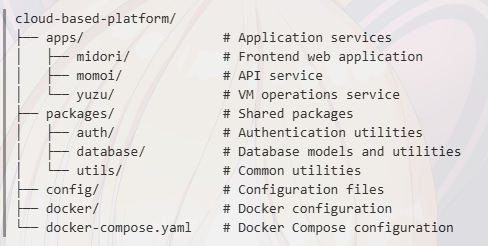
\includegraphics[width=0.8\textwidth]{Image/web/project_structure.png}
% }
% \caption{\fontSixTeen{โครงสร้างโครงงานทั้งหมด}}
% \label{fig4:ProjectStructure}
% \end{figure}

\hspace*{1.3em}
การจัดโครงสร้างโครงงานในลักษณะหลายรีโพซิทอรีนี้ช่วยให้สามารถกำหนดขอบเขตของบริการได้ชัดเจน ลดผลกระทบข้ามระบบเมื่อต้องแก้ไขโค้ด และเหมาะสมกับการดูแลระบบที่มีทั้ง application service และ deployment manifest อยู่ร่วมกันในแพลตฟอร์มเดียว

\section{สถาปัตยกรรมระบบและเทคโนโลยี}
\subsection{การออกแบบสถาปัตยกรรมแบบ Microservices}
\hspace*{1.3em}
ระบบแพลตฟอร์มคลาวด์ที่พัฒนาขึ้นใช้สถาปัตยกรรมแบบ Microservices ซึ่งประกอบด้วยบริการหลัก 3 ตัว คือ Midori, Momoi และ Yuzu โดยมีบริการสนับสนุนเพิ่มเติม เช่น PostgreSQL สำหรับข้อมูลธุรกรรม Redis สำหรับ cache และคิวงาน RustFS สำหรับพื้นที่จัดเก็บไฟล์ และชุด observability สำหรับติดตามสถานะของระบบ แต่ละบริการทำงานอิสระและสื่อสารกันผ่าน HTTP API และระบบคิวงานแบบ asynchronous เพื่อให้ระบบมีความยืดหยุ่นและรองรับการขยายตัวได้ง่าย

\hspace*{1.3em}
เมื่อพิจารณาการทำงานจริงของระบบในคลัสเตอร์ ผู้ใช้จะเริ่มจาก Browser ไปยัง Midori จากนั้น Midori จะเรียก Momoi สำหรับทั้ง API ด้านข้อมูล ตรรกะทางธุรกิจ และการยืนยันตัวตนผ่านเส้นทาง `/api/auth` ขณะที่ Momoi จะทำหน้าที่บันทึกข้อมูลธุรกรรมและส่งงานระยะยาวเข้าสู่ BullMQ บน Redis แล้วให้ Yuzu รับงานไปดำเนินการต่อกับ Proxmox VE รูปแบบนี้ทำให้ API หลักตอบสนองต่อผู้ใช้ได้รวดเร็ว แม้งานโครงสร้างพื้นฐานจะใช้เวลานานและต้อง retry หลายครั้ง

\hspace*{1.3em}
ภาพที่ \ref{fig4:SystemArchitecture} แสดงสถาปัตยกรรมระบบโดยรวม โดยมี \textbf{Midori} เป็นส่วนติดต่อผู้ใช้ที่พัฒนาด้วย Next.js และ React \textbf{Momoi} เป็นบริการ API หลักที่รับผิดชอบตรรกะทางธุรกิจ การเชื่อมต่อฐานข้อมูล และการส่งงานเข้าคิว \textbf{Yuzu} เป็นบริการประมวลผลงานจัดการเครื่องเสมือนที่เชื่อมต่อกับ Proxmox VE และ \textbf{Yuuka} เป็นแหล่งเก็บไฟล์กำหนดค่าการติดตั้งบริการประกอบทั้งหมดของแพลตฟอร์ม

\begin{figure}[H]
\centering
\adjustbox{frame, width=0.75\textwidth}{
    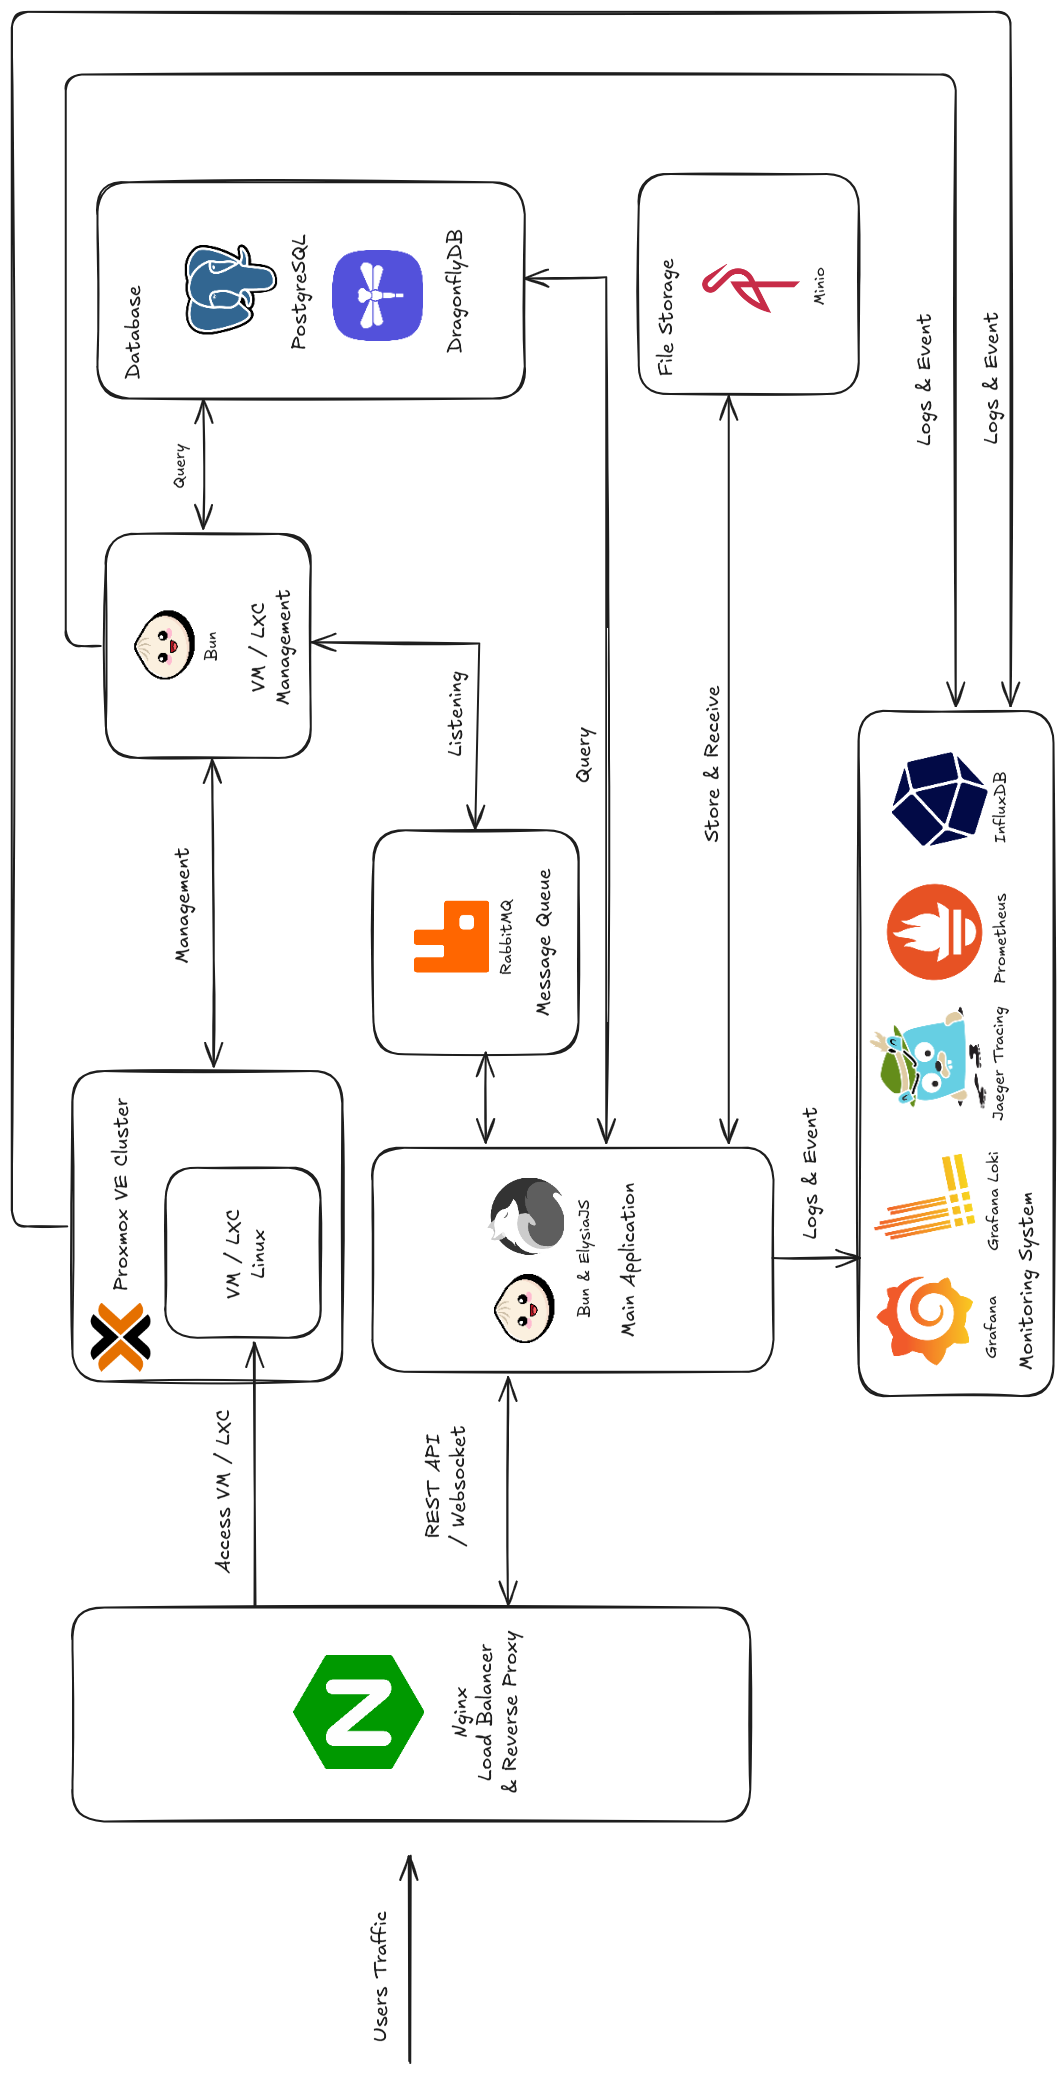
\includegraphics[width=0.75\textwidth]{Image/diagram/system_architecture_90.png}
}
\caption{\fontSixTeen{สถาปัตยกรรมระบบโดยรวม}}
\label{fig4:SystemArchitecture}
\end{figure}

\subsection{เทคโนโลยีที่ใช้ในการพัฒนา}
\hspace*{1.3em}
ในการพัฒนาระบบแพลตฟอร์มคลาวด์นี้ ได้เลือกใช้เทคโนโลยีที่ทันสมัยและเหมาะสมกับการใช้งานในสภาพแวดล้อมการศึกษา โดยเทคโนโลยีหลักที่ใช้ประกอบด้วย
\begin{mycustomitem}
    \item \textbf{Bun Runtime} - JavaScript/TypeScript Runtime ที่มีประสิทธิภาพสูง
    \item \textbf{Next.js 16 และ React 19} - Framework และ Library สำหรับการพัฒนา Frontend
    \item \textbf{Tailwind CSS และ Radix UI} - เครื่องมือสำหรับออกแบบส่วนติดต่อผู้ใช้
    \item \textbf{Elysia.js} - Web Framework สำหรับการพัฒนา API ของ Momoi
    \item \textbf{PostgreSQL} - ระบบจัดการฐานข้อมูลเชิงสัมพันธ์
    \item \textbf{Prisma ORM} - Object-Relational Mapping สำหรับการจัดการฐานข้อมูล
    \item \textbf{Redis และ BullMQ} - ระบบ cache และคิวงาน
    \item \textbf{Docker และ Kubernetes Manifests} - สำหรับการ deploy
    \item \textbf{Prometheus, Grafana, Loki และ Jaeger} - สำหรับการเก็บ metrics, logs และ traces
\end{mycustomitem}

\hspace*{1.3em}
การเลือกใช้เทคโนโลยีเหล่านี้มีเหตุผลสำคัญ คือ ความเสถียร ประสิทธิภาพ และการรองรับการขยายระบบในอนาคต รวมถึงการมี Community ที่ใหญ่และเอกสารประกอบที่ครบถ้วน ทำให้การพัฒนาและบำรุงรักษาระบบเป็นไปอย่างราบรื่น

\section{เอกสารประกอบการใช้งาน API และส่วนติดต่อผู้ใช้}
\subsection{เอกสาร API Documentation}
\hspace*{1.3em}
ระบบแพลตฟอร์มคลาวด์ได้จัดทำเอกสาร API Documentation อย่างครบถ้วนโดยใช้ OpenAPI Specification (Swagger) เพื่อให้ผู้พัฒนาและผู้ใช้งานสามารถเข้าใจและใช้งาน API ได้อย่างง่ายดาย เอกสารนี้ประกอบด้วยรายละเอียดของ Endpoints ต่าง ๆ พารามิเตอร์ที่ต้องการ รูปแบบข้อมูลที่ส่งและรับ รวมทั้งตัวอย่างการใช้งานที่ชัดเจน

\hspace*{1.3em}
ภาพที่ \ref{fig4:APIDocumentation} แสดงหน้าเอกสาร API Documentation ที่สร้างขึ้นโดยอัตโนมัติจากโค้ด TypeScript ผ่าน Elysia.js และ OpenAPI Plugin ซึ่งช่วยให้เห็นโครงสร้างของบริการ Momoi ตามโดเมนงานหลักของระบบ โดยสามารถจัดกลุ่มการใช้งานได้ดังนี้

\begin{mycustomitem}
    \item \textbf{Public API} - สำหรับการใช้งานทั่วไปที่ไม่ต้องมีการยืนยันตัวตน
    \item \textbf{Academic Management API} - สำหรับจัดการรายวิชา ภาคการศึกษา และข้อมูลผู้สอน
    \item \textbf{Request Workflow API} - สำหรับสร้าง ตรวจสอบ และอนุมัติคำร้องขอเครื่องเสมือน
    \item \textbf{Instance API} - สำหรับจัดการเครื่องเสมือนและช่องทางเข้าถึงบริการ
    \item \textbf{Storage API} - สำหรับจัดการไฟล์
\end{mycustomitem}

\begin{figure}[htbp]
\centering
\adjustbox{frame, width=1.0\textwidth}{
    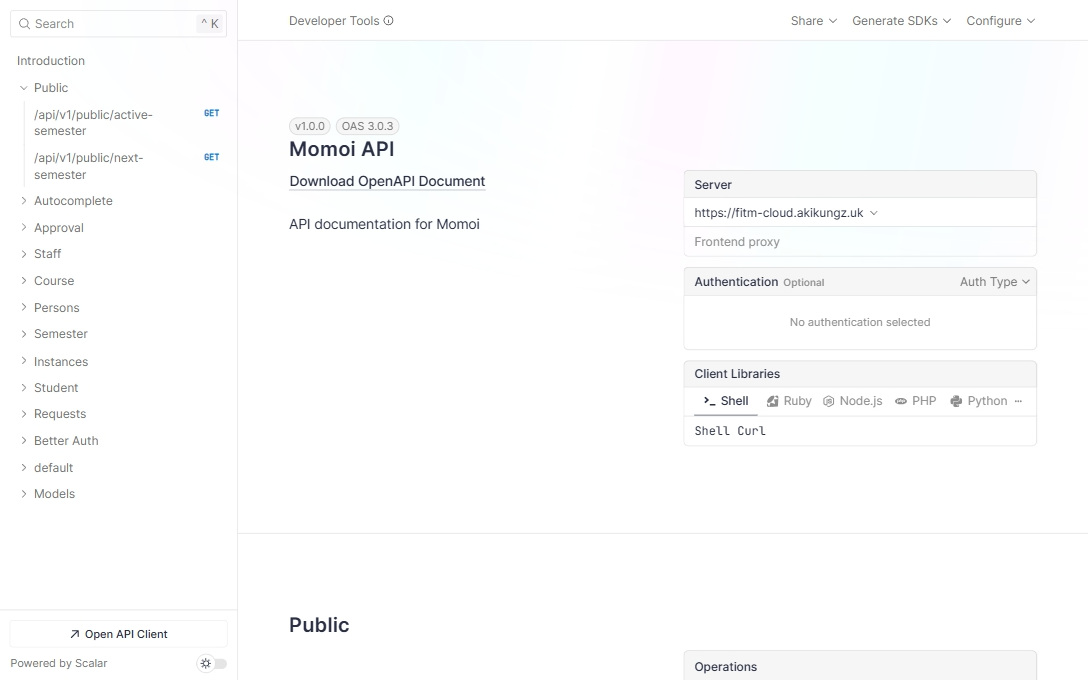
\includegraphics[width=1.0\textwidth]{Image/web/api_documentation.png}
}
\caption{\fontSixTeen{หน้าเอกสาร API Documentation}}
\label{fig4:APIDocumentation}
\end{figure}

\newpage
\hspace*{1.3em}
เอกสาร API นี้มีการอัปเดตอัตโนมัติเมื่อมีการเปลี่ยนแปลงโค้ด และสามารถทดสอบ API ได้โดยตรงผ่านหน้าเว็บ ทำให้ผู้พัฒนาสามารถทำความเข้าใจและใช้งาน API ได้อย่างรวดเร็วและถูกต้อง

\subsection{ส่วนติดต่อผู้ใช้ (User Interface)}
\hspace*{1.3em}
ส่วนติดต่อผู้ใช้ของระบบได้รับการออกแบบให้ใช้งานง่าย สวยงาม และตอบสนองได้ดีบนอุปกรณ์ต่าง ๆ โดยพัฒนาด้วย Next.js, React, Tailwind CSS และชุดองค์ประกอบ UI ที่อิงกับ Radix UI ระบบประกอบด้วยหน้าหลักต่าง ๆ ที่มีการจัดระเบียบข้อมูลและฟังก์ชันการทำงานอย่างชัดเจน ทั้งในส่วนของ dashboard, request workflow, instance management และ storage interface

\hspace*{1.3em}
ภาพที่ \ref{fig4:LandingPage} แสดงหน้าแรกของระบบ (Landing Page) ที่ออกแบบให้ดึงดูดความสนใจและสื่อสารจุดประสงค์ของระบบได้ชัดเจน โดยมีการนำเสนอฟีเจอร์หลักของระบบ ข้อมูลการติดต่อ และลิงก์สำหรับการล็อกอินเข้าสู่ระบบ

\begin{figure}[H]
\centering
\adjustbox{frame, width=0.8\textwidth}{
    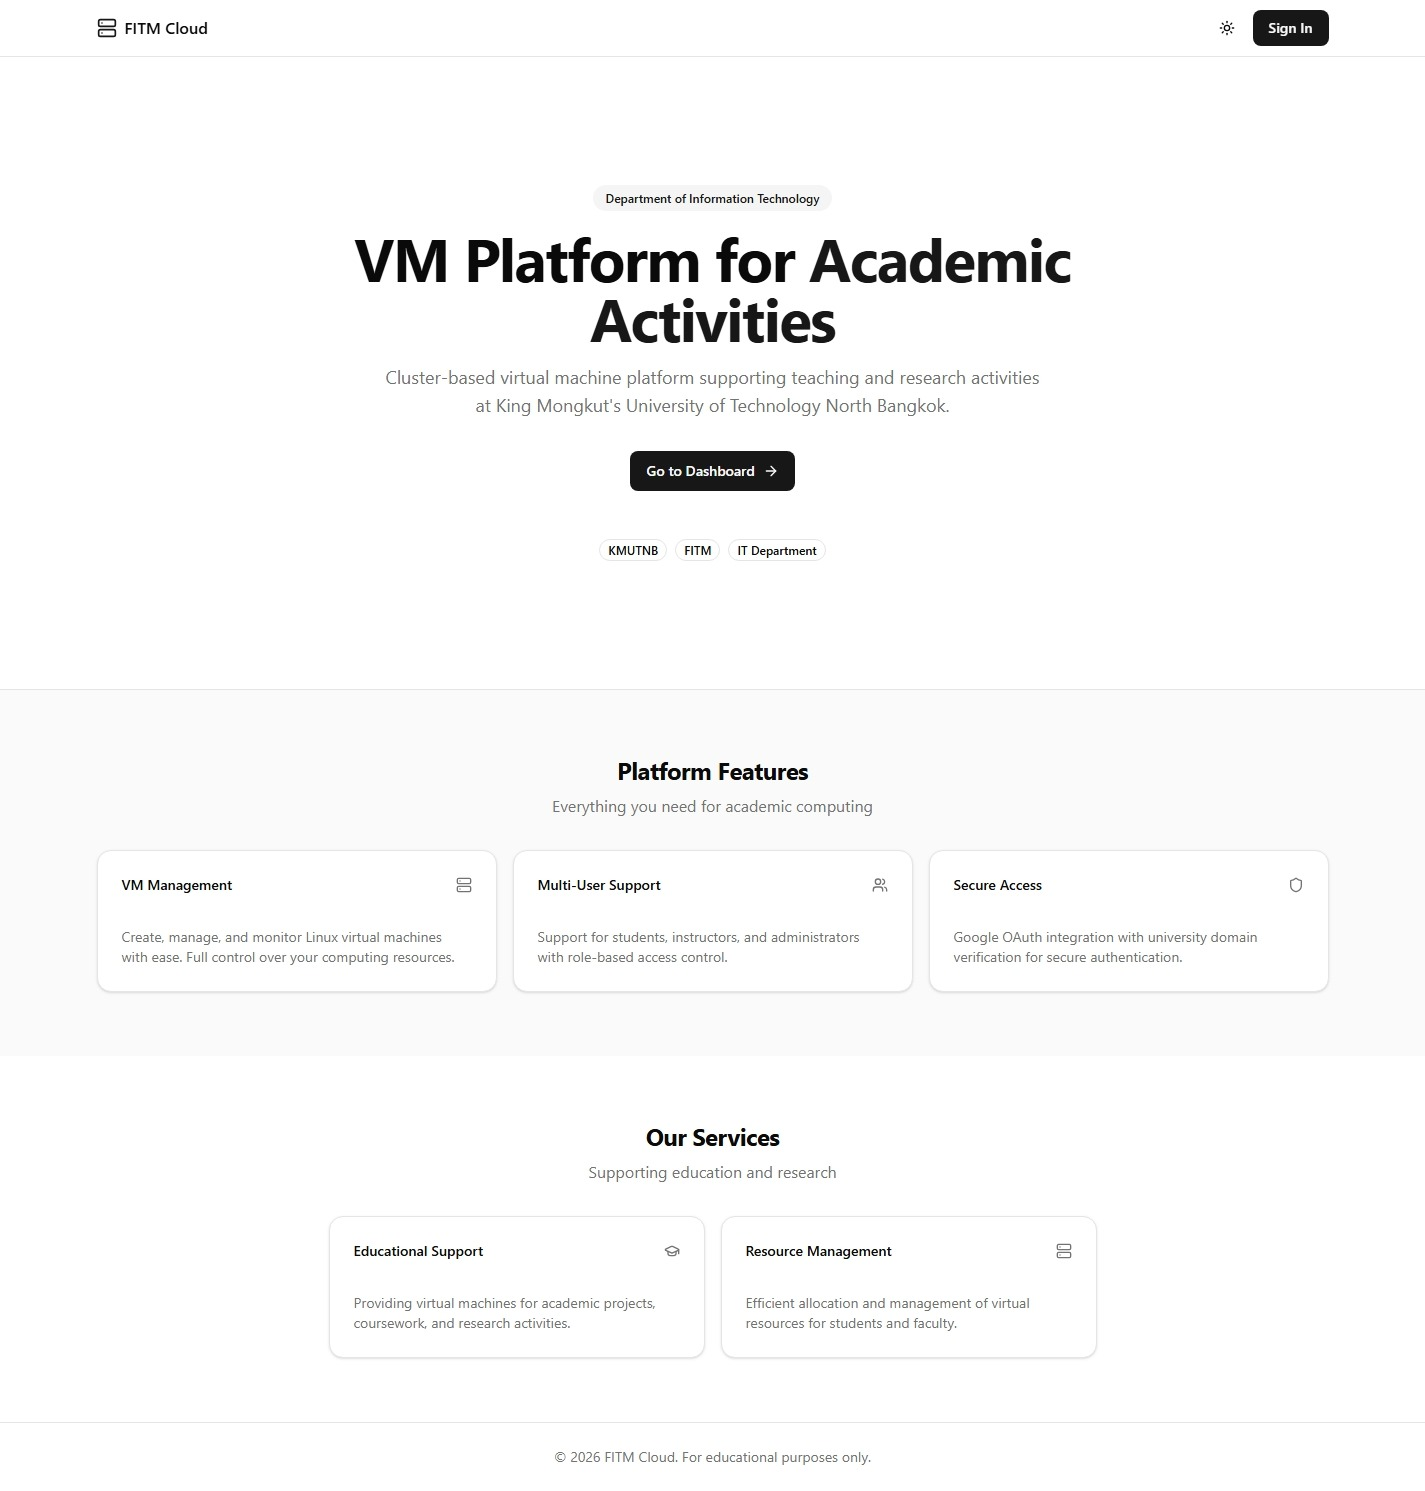
\includegraphics[width=1.0\textwidth]{Image/web/landing_page.jpeg}
}
\caption{\fontSixTeen{หน้าแรกของระบบ (Landing Page)}}
\label{fig4:LandingPage}
\end{figure}

% \newpage
\subsection{Dashboard และระบบจัดการ}
\hspace*{1.3em}
หลังจากที่ผู้ใช้ล็อกอินเข้าสู่ระบบแล้ว ผู้ใช้จะเข้าสู่หน้า Dashboard ที่แสดงข้อมูลสำคัญและฟังก์ชันการทำงานต่าง ๆ ตามบทบาทของผู้ใช้ โดย Dashboard ได้รับการออกแบบให้แสดงข้อมูลอย่างเป็นระบบและเข้าใจง่าย พร้อมทั้งมีการใช้งานที่สะดวกและรวดเร็ว

\hspace*{1.3em}
ส่วนติดต่อผู้ใช้ที่พัฒนาขึ้นมีลักษณะสำคัญดังนี้
\begin{mycustomitem}
    \item \textbf{Responsive Design} - รองรับการแสดงผลบนหน้าจอขนาดต่าง ๆ
    \item \textbf{Intuitive Navigation} - การนำทางที่เข้าใจง่ายและสอดคล้องกับมาตรฐาน UX
    \item \textbf{Role-based UI Visibility} - เมนูและตัวเลือกปรับแสดงผลโดยอัตโนมัติตามบทบาทของผู้ใช้ STUDENT INSTRUCTOR หรือ ADMIN โดยไม่ต้องกำหนดเพิ่มเติม
    \item \textbf{Request Lifecycle Tracking} - แสดงสถานะคำร้องขอตั้งแต่การยื่น การรอพิจารณา จนถึงการอนุมัติหรือปฏิเสธ พร้อม Audit Log ในแต่ละขั้นตอน
    \item \textbf{Instance Control Panel} - แผงควบคุมสถานะเครื่องเสมือน รองรับการสั่ง Start Stop Restart และดูข้อมูล IP และ Reverse Proxy ได้จากหน้าเดียวกัน
    \item \textbf{File Management Interface} - อินเทอร์เฟซสำหรับอัปโหลด จัดโฟลเดอร์ และกำหนดสิทธิ์การแบ่งปันไฟล์ภายในแพลตฟอร์ม
\end{mycustomitem}

\hspace*{1.3em}
การออกแบบส่วนติดต่อผู้ใช้ได้คำนึงถึงประสบการณ์ผู้ใช้ (User Experience) เป็นหลัก โดยมุ่งเน้นให้ผู้ใช้สามารถทำงานได้อย่างมีประสิทธิภาพและลดข้อผิดพลาดในการใช้งาน ทั้งนี้ระบบยังมีการจัดการข้อผิดพลาดและการแจ้งเตือนที่ชัดเจน เพื่อให้ผู้ใช้สามารถแก้ไขปัญหาได้อย่างรวดเร็ว

\section{ตัวอย่างการใช้งานระบบตามบทบาทผู้ใช้}
\subsection{Dashboard สำหรับนักศึกษา}
\hspace*{1.3em}
ระบบได้จัดทำ Dashboard เฉพาะสำหรับนักศึกษา เพื่อให้สามารถจัดการเครื่องเสมือนส่วนตัวและติดตามการใช้งานทรัพยากรได้อย่างง่ายดาย ภาพที่ \ref{fig4:StudentDashboard} แสดง Dashboard หลักของนักศึกษาที่ประกอบด้วยข้อมูลสรุปการใช้งาน สถานะเครื่องเสมือน และฟังก์ชันการจัดการที่สำคัญ

\begin{figure}[H]
\centering
\adjustbox{frame, width=0.8\textwidth}{
    
\includegraphics[width=1.0\textwidth]{Image/web/dashboard/student/dashboard.jpeg}
}
\caption{\fontSixTeen{Dashboard หลักสำหรับนักศึกษา}}
\label{fig4:StudentDashboard}
\end{figure}

\hspace*{1.3em}
นักศึกษาสามารถดูรายการเครื่องเสมือนทั้งหมดที่ตนเองมีสิทธิ์เข้าถึง พร้อมทั้งสถานะการทำงาน การใช้ทรัพยากร และการจัดการพื้นฐาน ดังแสดงในภาพที่ \ref{fig4:StudentInstances} ซึ่งนำเสนอรายละเอียดของแต่ละ Instance อย่างชัดเจน

\begin{figure}[H]
\centering
\adjustbox{frame, width=0.8\textwidth}{
    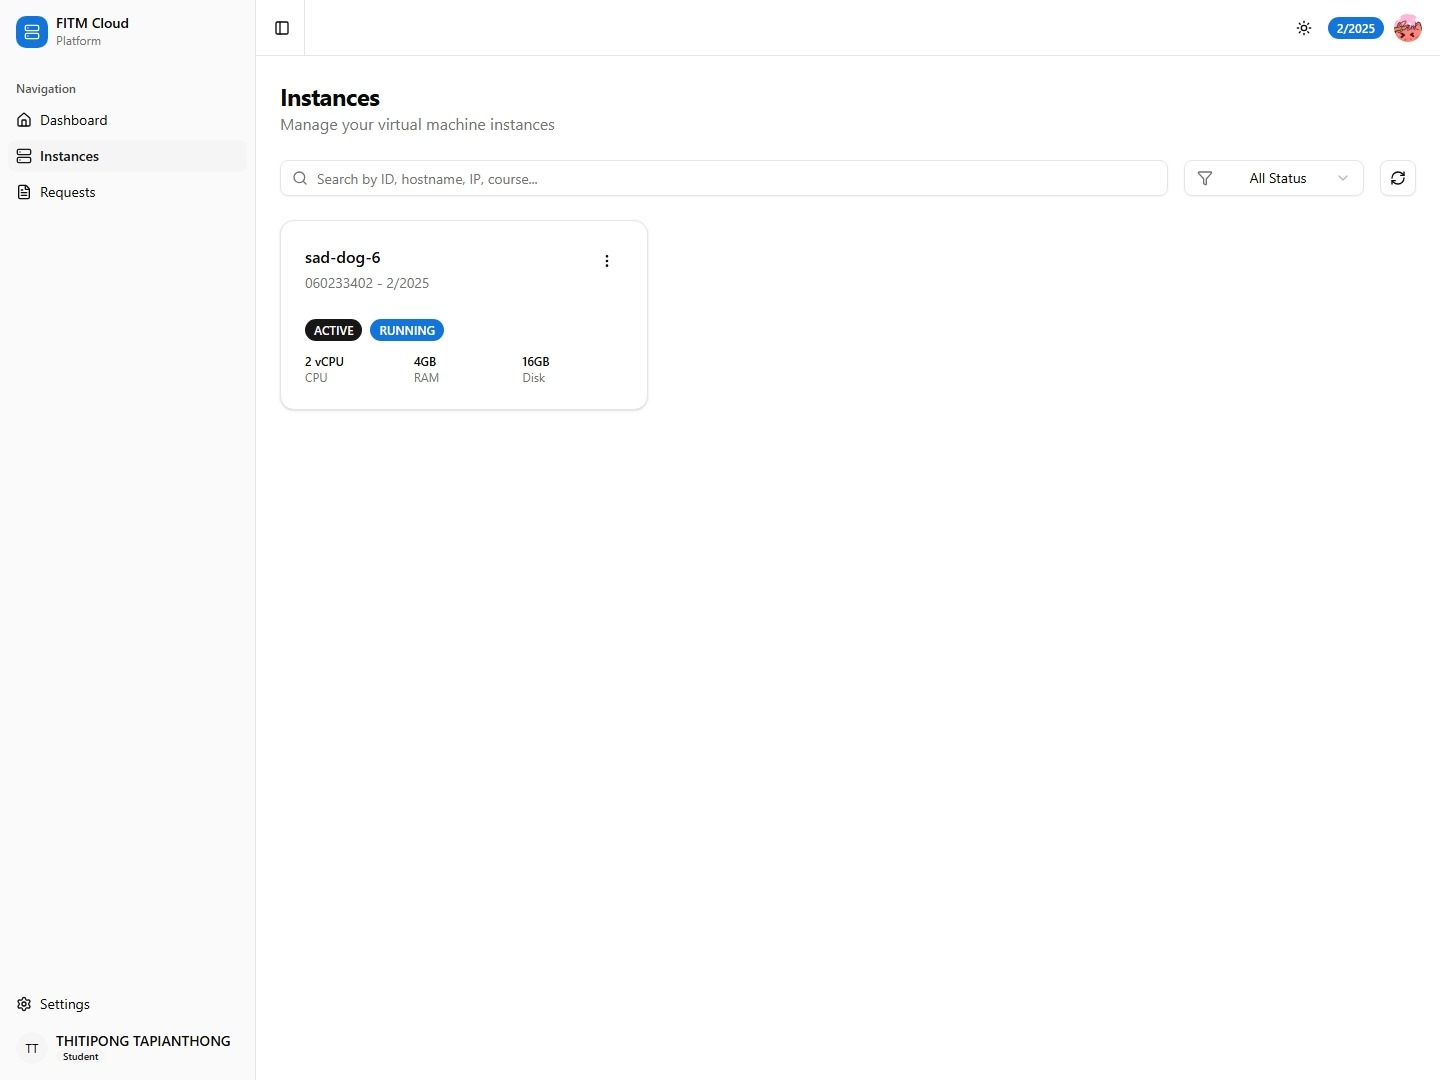
\includegraphics[width=1.0\textwidth]{Image/web/dashboard/student/instances.jpeg}
}
\caption{\fontSixTeen{หน้าจัดการ VM Instances สำหรับนักศึกษา}}
\label{fig4:StudentInstances}
\end{figure}

\hspace*{1.3em}
นอกจากนี้ นักศึกษายังสามารถขอสร้างเครื่องเสมือนใหม่ผ่านฟอร์มที่ออกแบบมาอย่างเรียบง่าย ดังแสดงในภาพที่ \ref{fig4:StudentCreateInstance} ซึ่งช่วยให้การขอใช้ทรัพยากรเป็นไปอย่างรวดเร็วและมีประสิทธิภาพ

\begin{figure}[H]
\centering
\adjustbox{frame, width=0.8\textwidth}{
    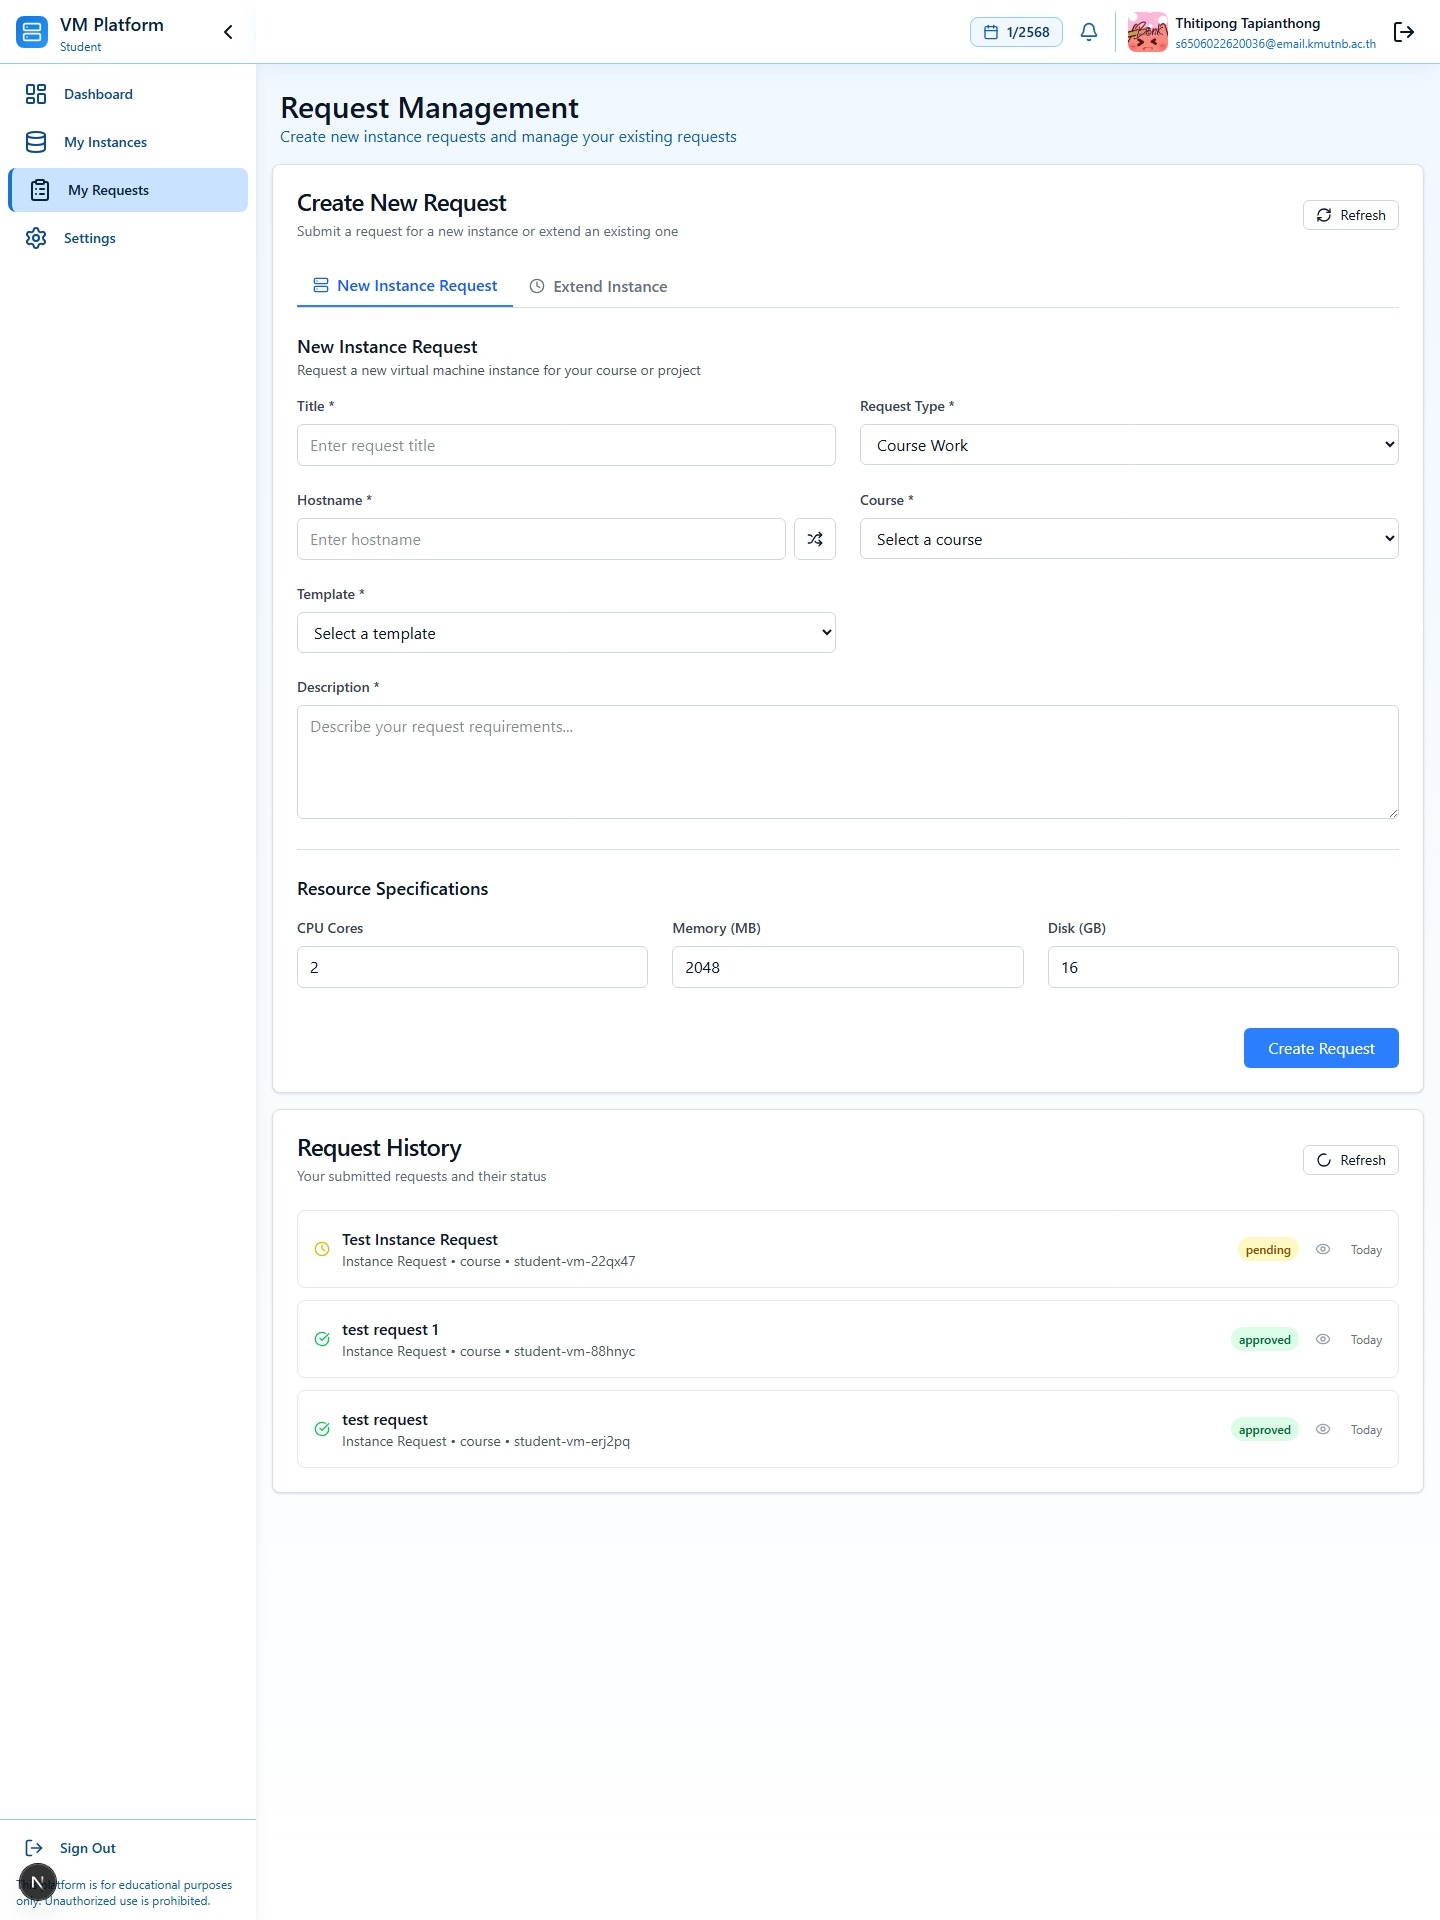
\includegraphics[width=1.0\textwidth]{Image/web/dashboard/student/requests.jpeg}
}
\caption{\fontSixTeen{หน้าจอขอสร้าง VM Instance ใหม่สำหรับนักศึกษา}}
\label{fig4:StudentCreateInstance}
\end{figure}

\newpage
\subsection{Dashboard สำหรับอาจารย์และเจ้าหน้าที่}
\hspace*{1.3em}
สำหรับอาจารย์และเจ้าหน้าที่ ระบบได้จัดเตรียม Dashboard ที่มีฟังก์ชันการจัดการขั้นสูงมากขึ้น รวมถึงการอนุมัติคำขอ การจัดการหลักสูตร และการตรวจสอบการใช้งานของนักศึกษา ภาพที่ \ref{fig4:StaffDashboard} แสดง Dashboard หลักสำหรับเจ้าหน้าที่ที่มีข้อมูลสถิติและการควบคุมระบบ

\begin{figure}[H]
\centering
\adjustbox{frame, width=0.8\textwidth}{
    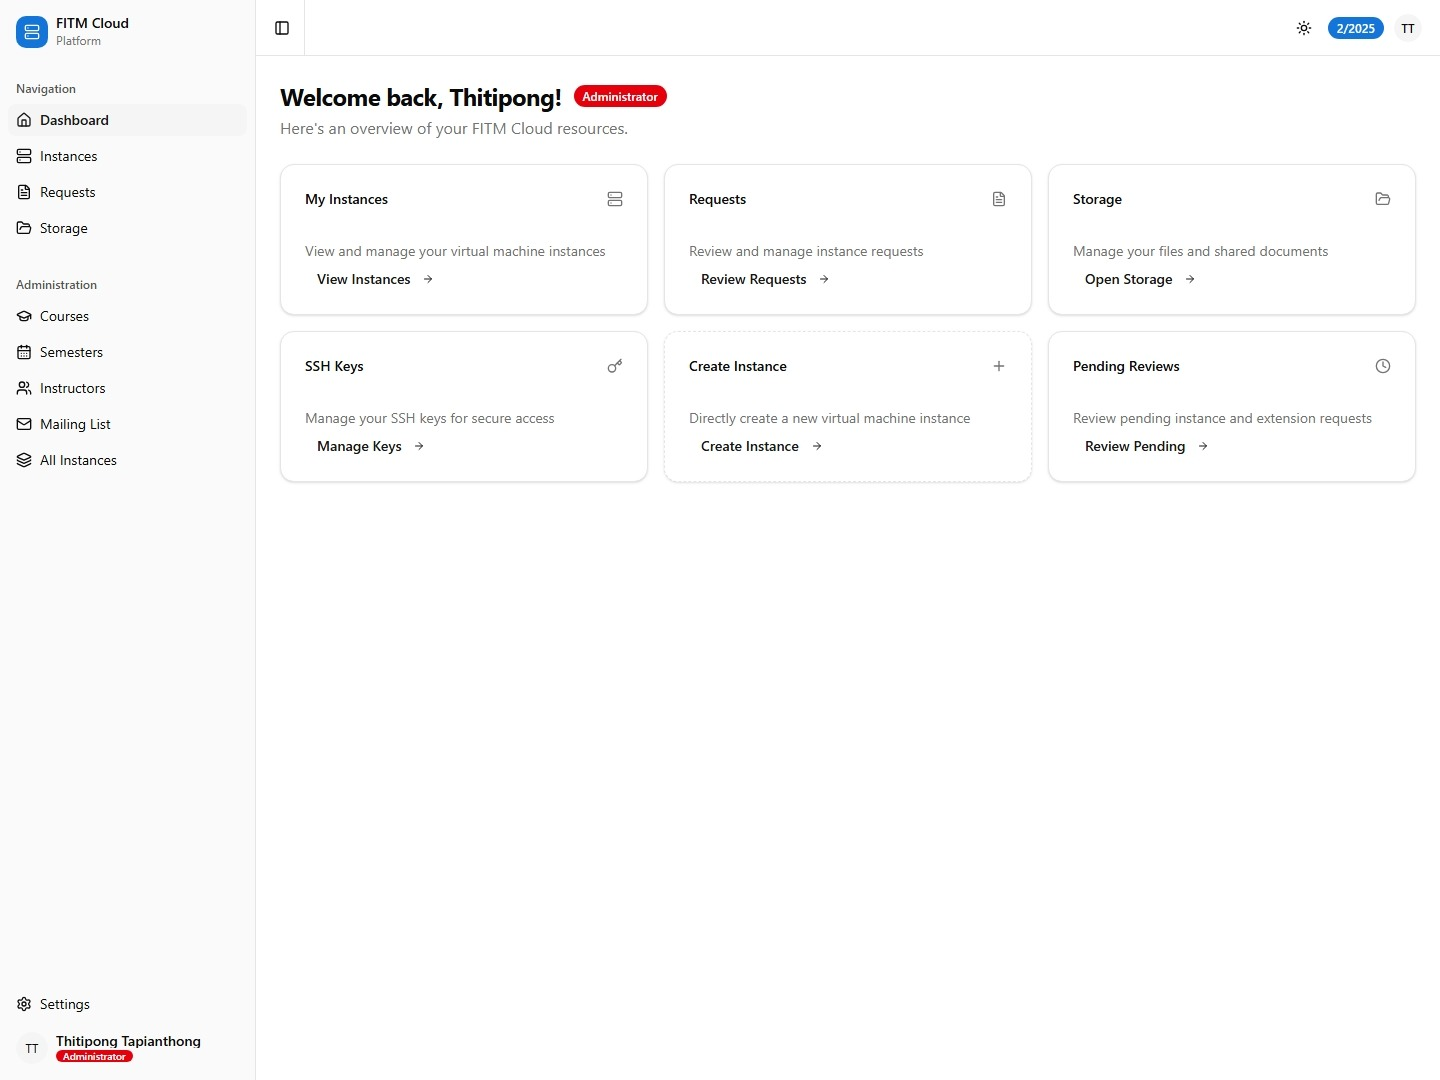
\includegraphics[width=1.0\textwidth]{Image/web/dashboard/staff/dashboard.jpeg}
}
\caption{\fontSixTeen{Dashboard หลักสำหรับอาจารย์และเจ้าหน้าที่}}
\label{fig4:StaffDashboard}
\end{figure}

\hspace*{1.3em}
อาจารย์และเจ้าหน้าที่สามารถจัดการหลักสูตร เทอมการศึกษา รวมถึงการจัดการรายชื่อของอาจารย์และเจ้าหน้าที่ ดังแสดงในภาพที่ \ref{fig4:CourseManagement} - \ref{fig4:StaffManagement} ซึ่งช่วยให้สามารถกำหนดทรัพยากรและสิทธิ์การเข้าถึงสำหรับแต่ละวิชาได้อย่างเหมาะสม

\begin{figure}[H]
\centering
\adjustbox{frame, width=0.8\textwidth}{
    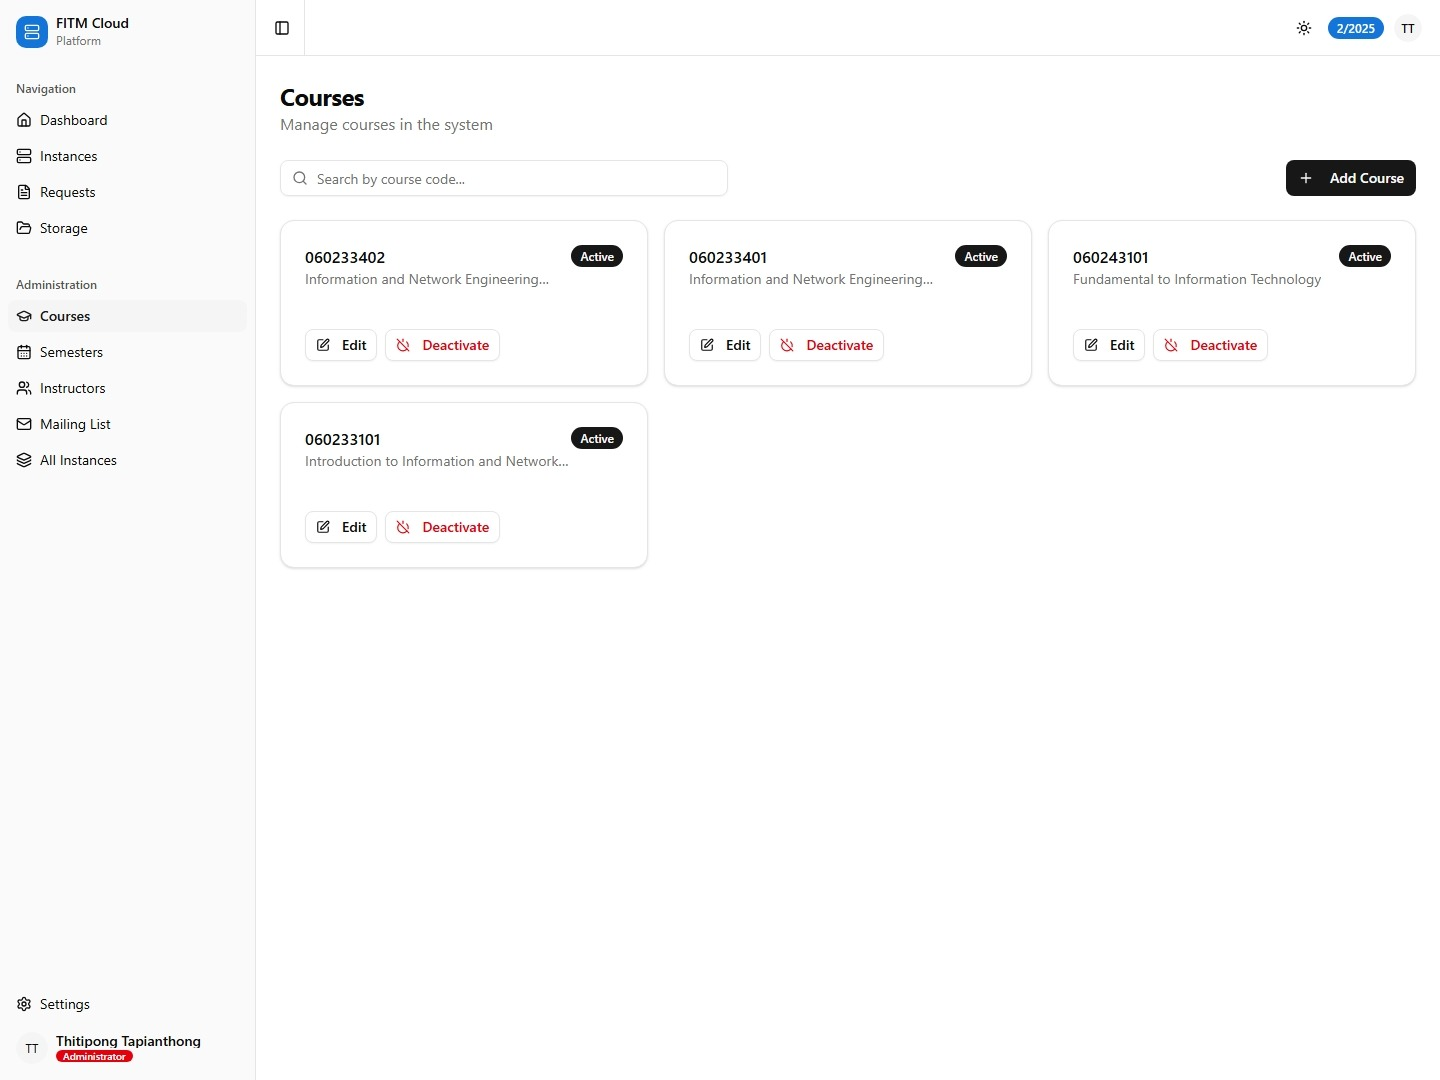
\includegraphics[width=0.8\textwidth]{Image/web/dashboard/staff/courses.jpeg}
}
\caption{\fontSixTeen{หน้าจัดการหลักสูตรและรายวิชา}}
\label{fig4:CourseManagement}
\end{figure}

\begin{figure}[H]
\centering
\adjustbox{frame, width=0.8\textwidth}{
    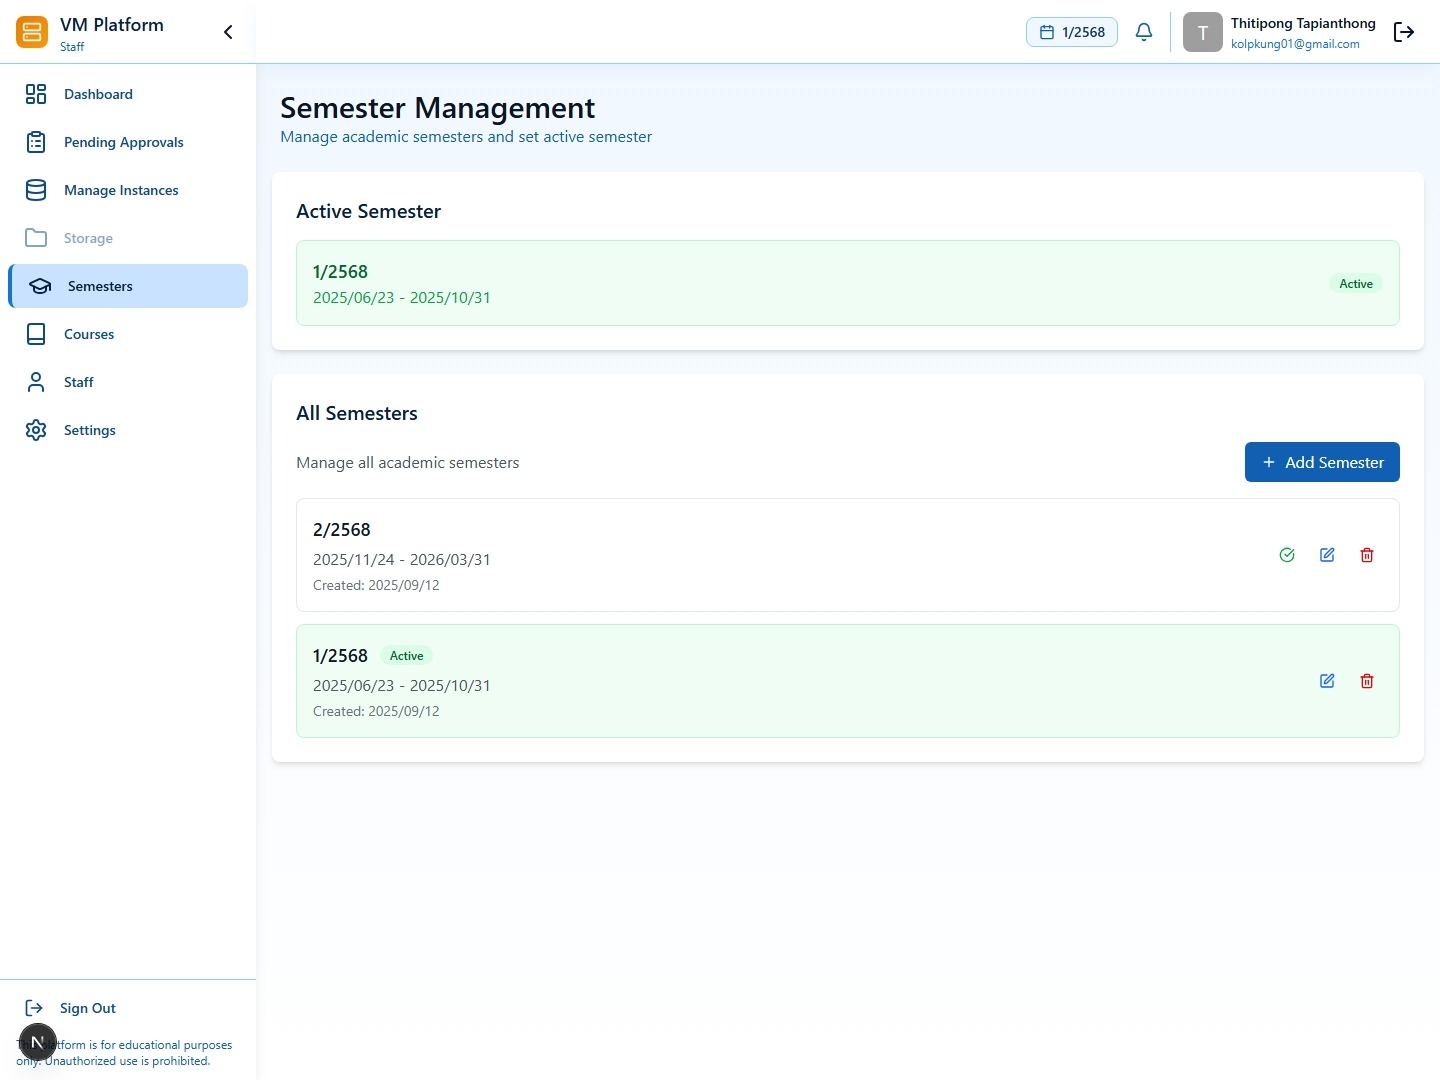
\includegraphics[width=0.8\textwidth]{Image/web/dashboard/staff/semesters.jpeg}
}
\caption{\fontSixTeen{หน้าจัดการเทอมการศึกษา}}
\label{fig4:SemesterManagement}
\end{figure}

\begin{figure}[H]
\centering
\adjustbox{frame, width=0.8\textwidth}{
    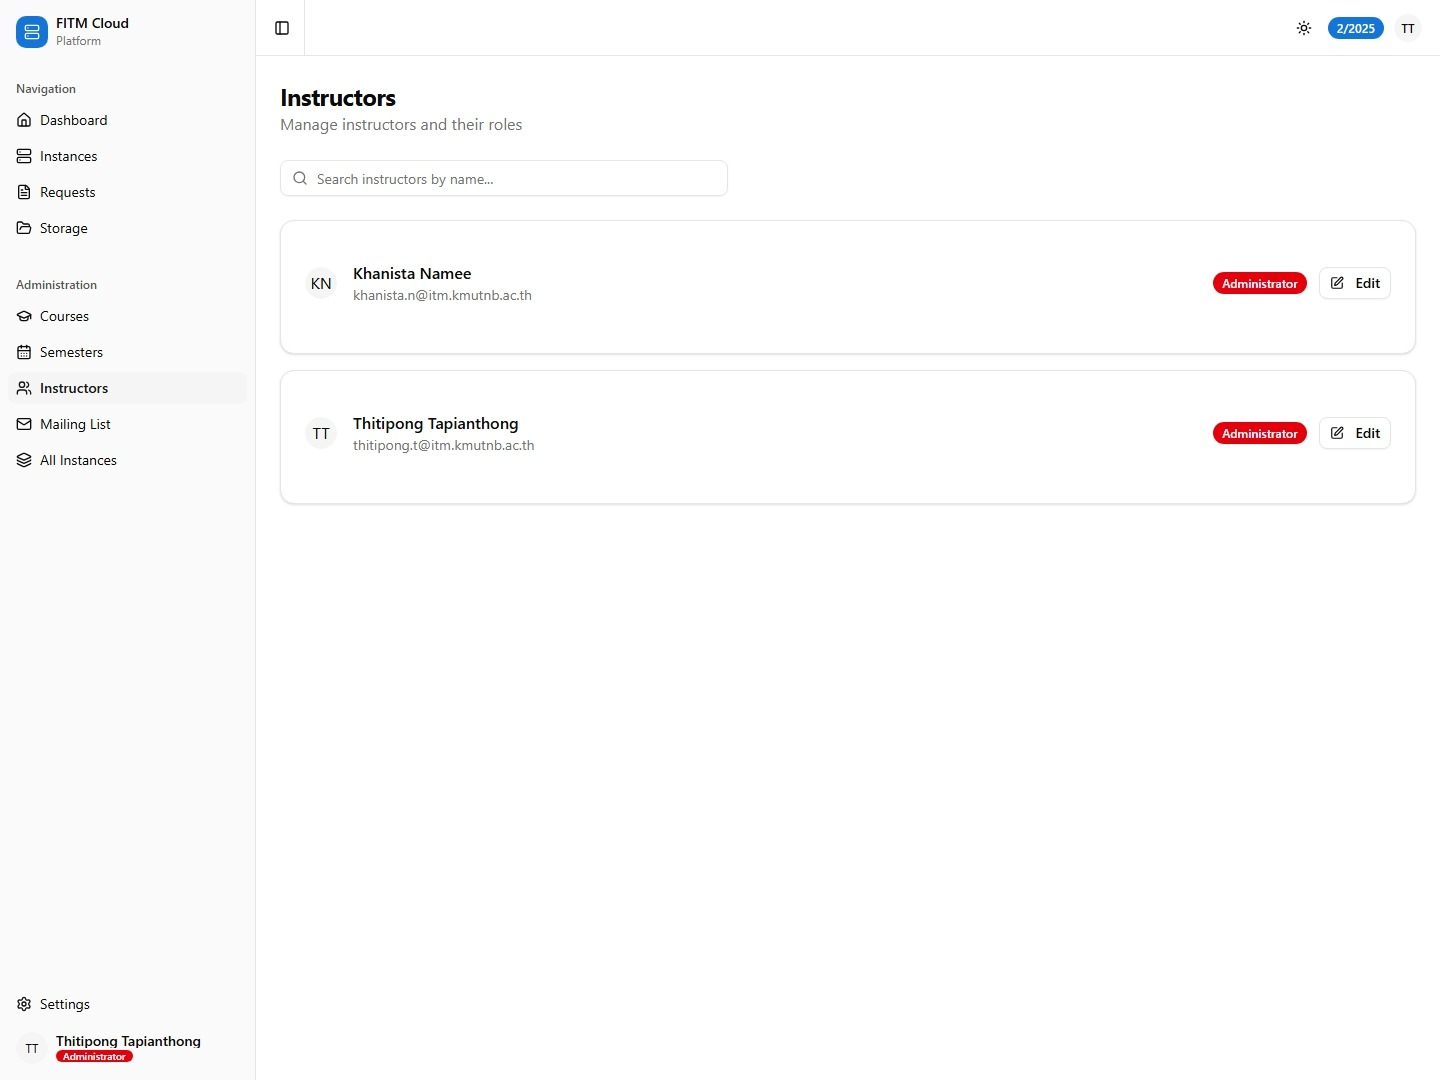
\includegraphics[width=0.8\textwidth]{Image/web/dashboard/staff/staff_management.jpeg}
}
\caption{\fontSixTeen{หน้าจัดการรายชื่ออาจารย์}}
\label{fig4:StaffManagement}
\end{figure}

\hspace*{1.3em}
นอกจากนี้ ระบบยังมีหน้าสำหรับการอนุมัติคำขอต่าง ๆ จากนักศึกษา ดังแสดงในภาพที่ \ref{fig4:PendingApproval} ซึ่งช่วยให้อาจารย์สามารถตรวจสอบและอนุมัติคำขอได้อย่างมีประสิทธิภาพ

\begin{figure}[H]
\centering
\adjustbox{frame, width=0.8\textwidth}{
    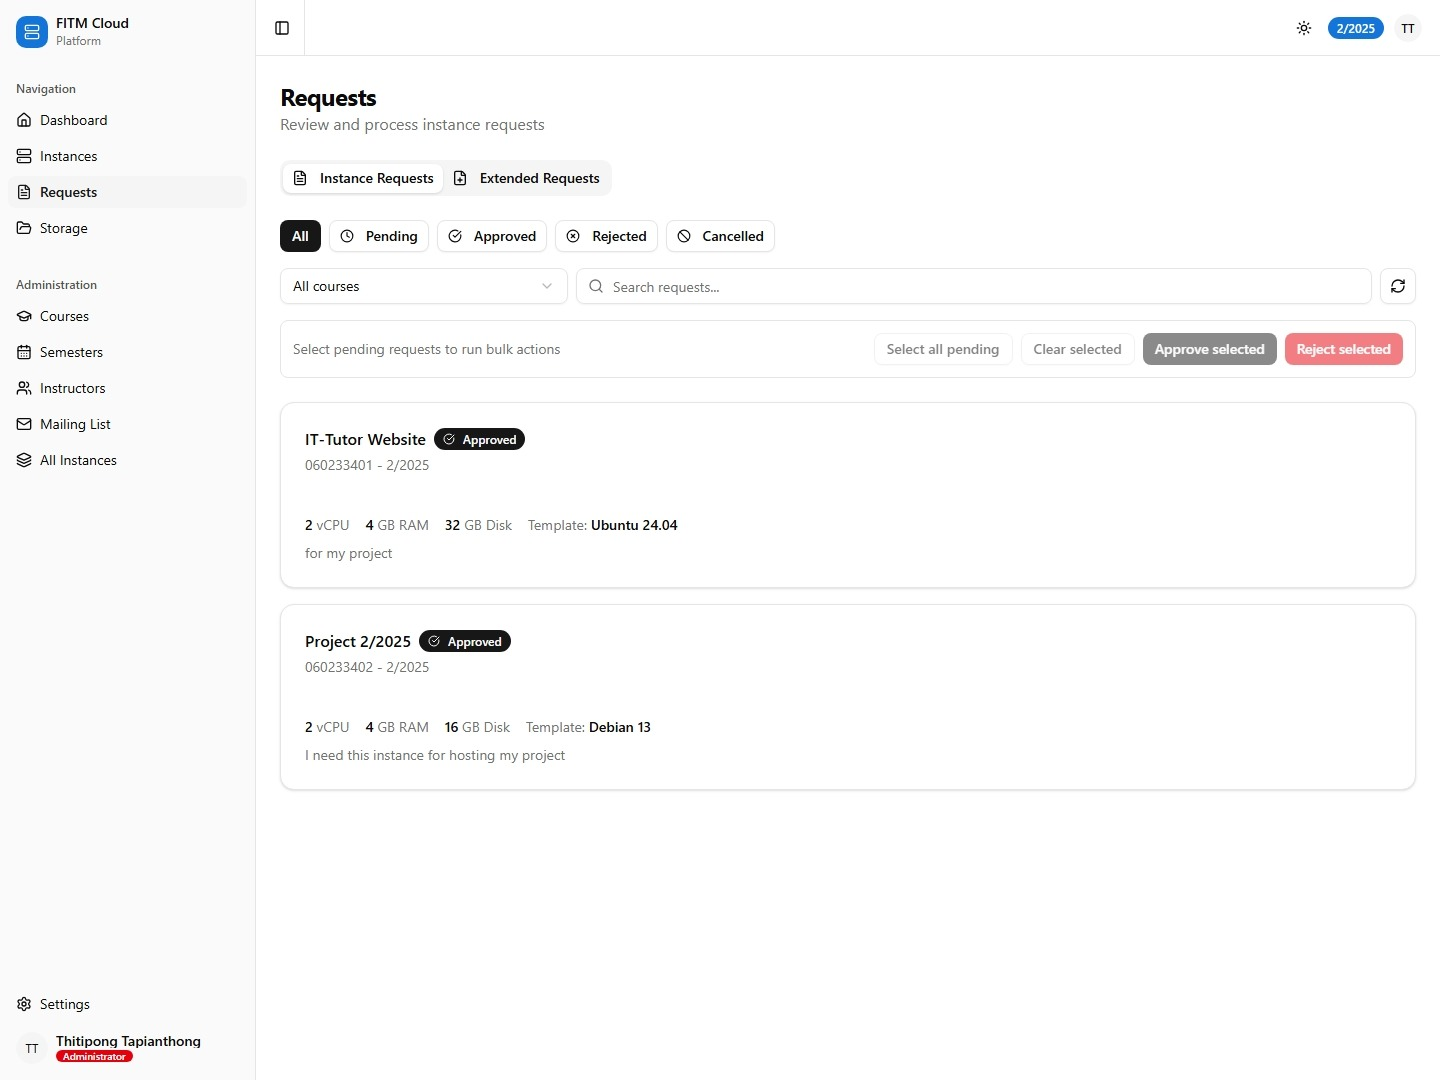
\includegraphics[width=0.8\textwidth]{Image/web/dashboard/staff/pending_approval.jpeg}
}
\caption{\fontSixTeen{หน้าอนุมัติคำขอที่รอดำเนินการ}}
\label{fig4:PendingApproval}
\end{figure}

% \newpage
\subsection{ระบบจัดการแบบ Role-Based Access Control}
\hspace*{1.3em}
ระบบได้นำเอา Role-Based Access Control (RBAC) มาใช้ในการจัดการสิทธิ์การเข้าถึงข้อมูลและฟังก์ชันต่าง ๆ โดยแบ่งผู้ใช้เป็น 3 กลุ่มหลัก คือ นักศึกษา อาจารย์ และผู้ดูแลระบบ ซึ่งแต่ละกลุ่มจะมีสิทธิ์และหน้าที่ที่แตกต่างกันตามความเหมาะสม

\hspace*{1.3em}
การออกแบบระบบในลักษณะนี้ช่วยให้การจัดการความปลอดภัยของข้อมูลเป็นไปอย่างมีประสิทธิภาพ และผู้ใช้แต่ละกลุ่มจะเห็นเฉพาะข้อมูลและฟังก์ชันที่เกี่ยวข้องกับหน้าที่ของตนเอง ทำให้การใช้งานง่ายขึ้นและลดความเสี่ยงในการเข้าถึงข้อมูลที่ไม่เหมาะสม

\section{ระบบติดตามและสังเกตการณ์การทำงาน (Observability)}
\hspace*{1.3em}
ระบบได้ติดตั้งชุดเครื่องมือสำหรับสังเกตการณ์การทำงาน (Observability Stack) โดยใช้ \textbf{Prometheus} สำหรับเก็บ metrics จากบริการหลัก \textbf{Grafana} สำหรับแสดงผลบนหน้า dashboard \textbf{Loki} สำหรับรวบรวมและค้นหา application log และ \textbf{Jaeger} สำหรับ distributed tracing ข้ามบริการ ทำให้ผู้ดูแลระบบสามารถติดตามสถานะและวิเคราะห์ปัญหาได้แบบ real-time

\subsection{ผลการติดตามบน Grafana Dashboard}
\hspace*{1.3em}
แต่ละบริการหลักมีรูปแบบการสังเกตการณ์ที่แตกต่างกันตามบทบาทของตนเอง โดย Midori และ Momoi มีการส่ง traces ไปยัง Jaeger ผ่าน OpenTelemetry และมี metrics endpoint สำหรับ Prometheus ส่วน Yuzu เน้นการเปิดเผย metrics และ structured logs ของ queue worker และการเรียกใช้งาน Proxmox VE ผ่าน Prometheus-compatible endpoint ของตนเอง ตัวชี้วัดหลักที่ติดตาม ได้แก่ อัตราคำขอต่อวินาที latency percentile (p50, p95, p99) สถานะของ queue worker จำนวนงานในคิว เวลาในการทำ provision และอัตราความสำเร็จของการจัดสรรเครื่องเสมือน ข้อมูลเหล่านี้จะถูกนำเสนอใน Grafana dashboard ที่ออกแบบแยกตามบริการ และรวมไว้ในหน้าภาพรวมของระบบทั้งหมด

\hspace*{1.3em}
ภาพที่ \ref{fig4:MonitoringDashboard} แสดงตัวอย่างผลการติดตามบน Grafana ซึ่งช่วยให้ผู้ดูแลระบบเห็นภาพรวมของสถานะบริการและแนวโน้มของตัวชี้วัดสำคัญได้ในหน้าเดียว

\begin{figure}[H]
\centering
\adjustbox{frame, width=0.5\textwidth}{
    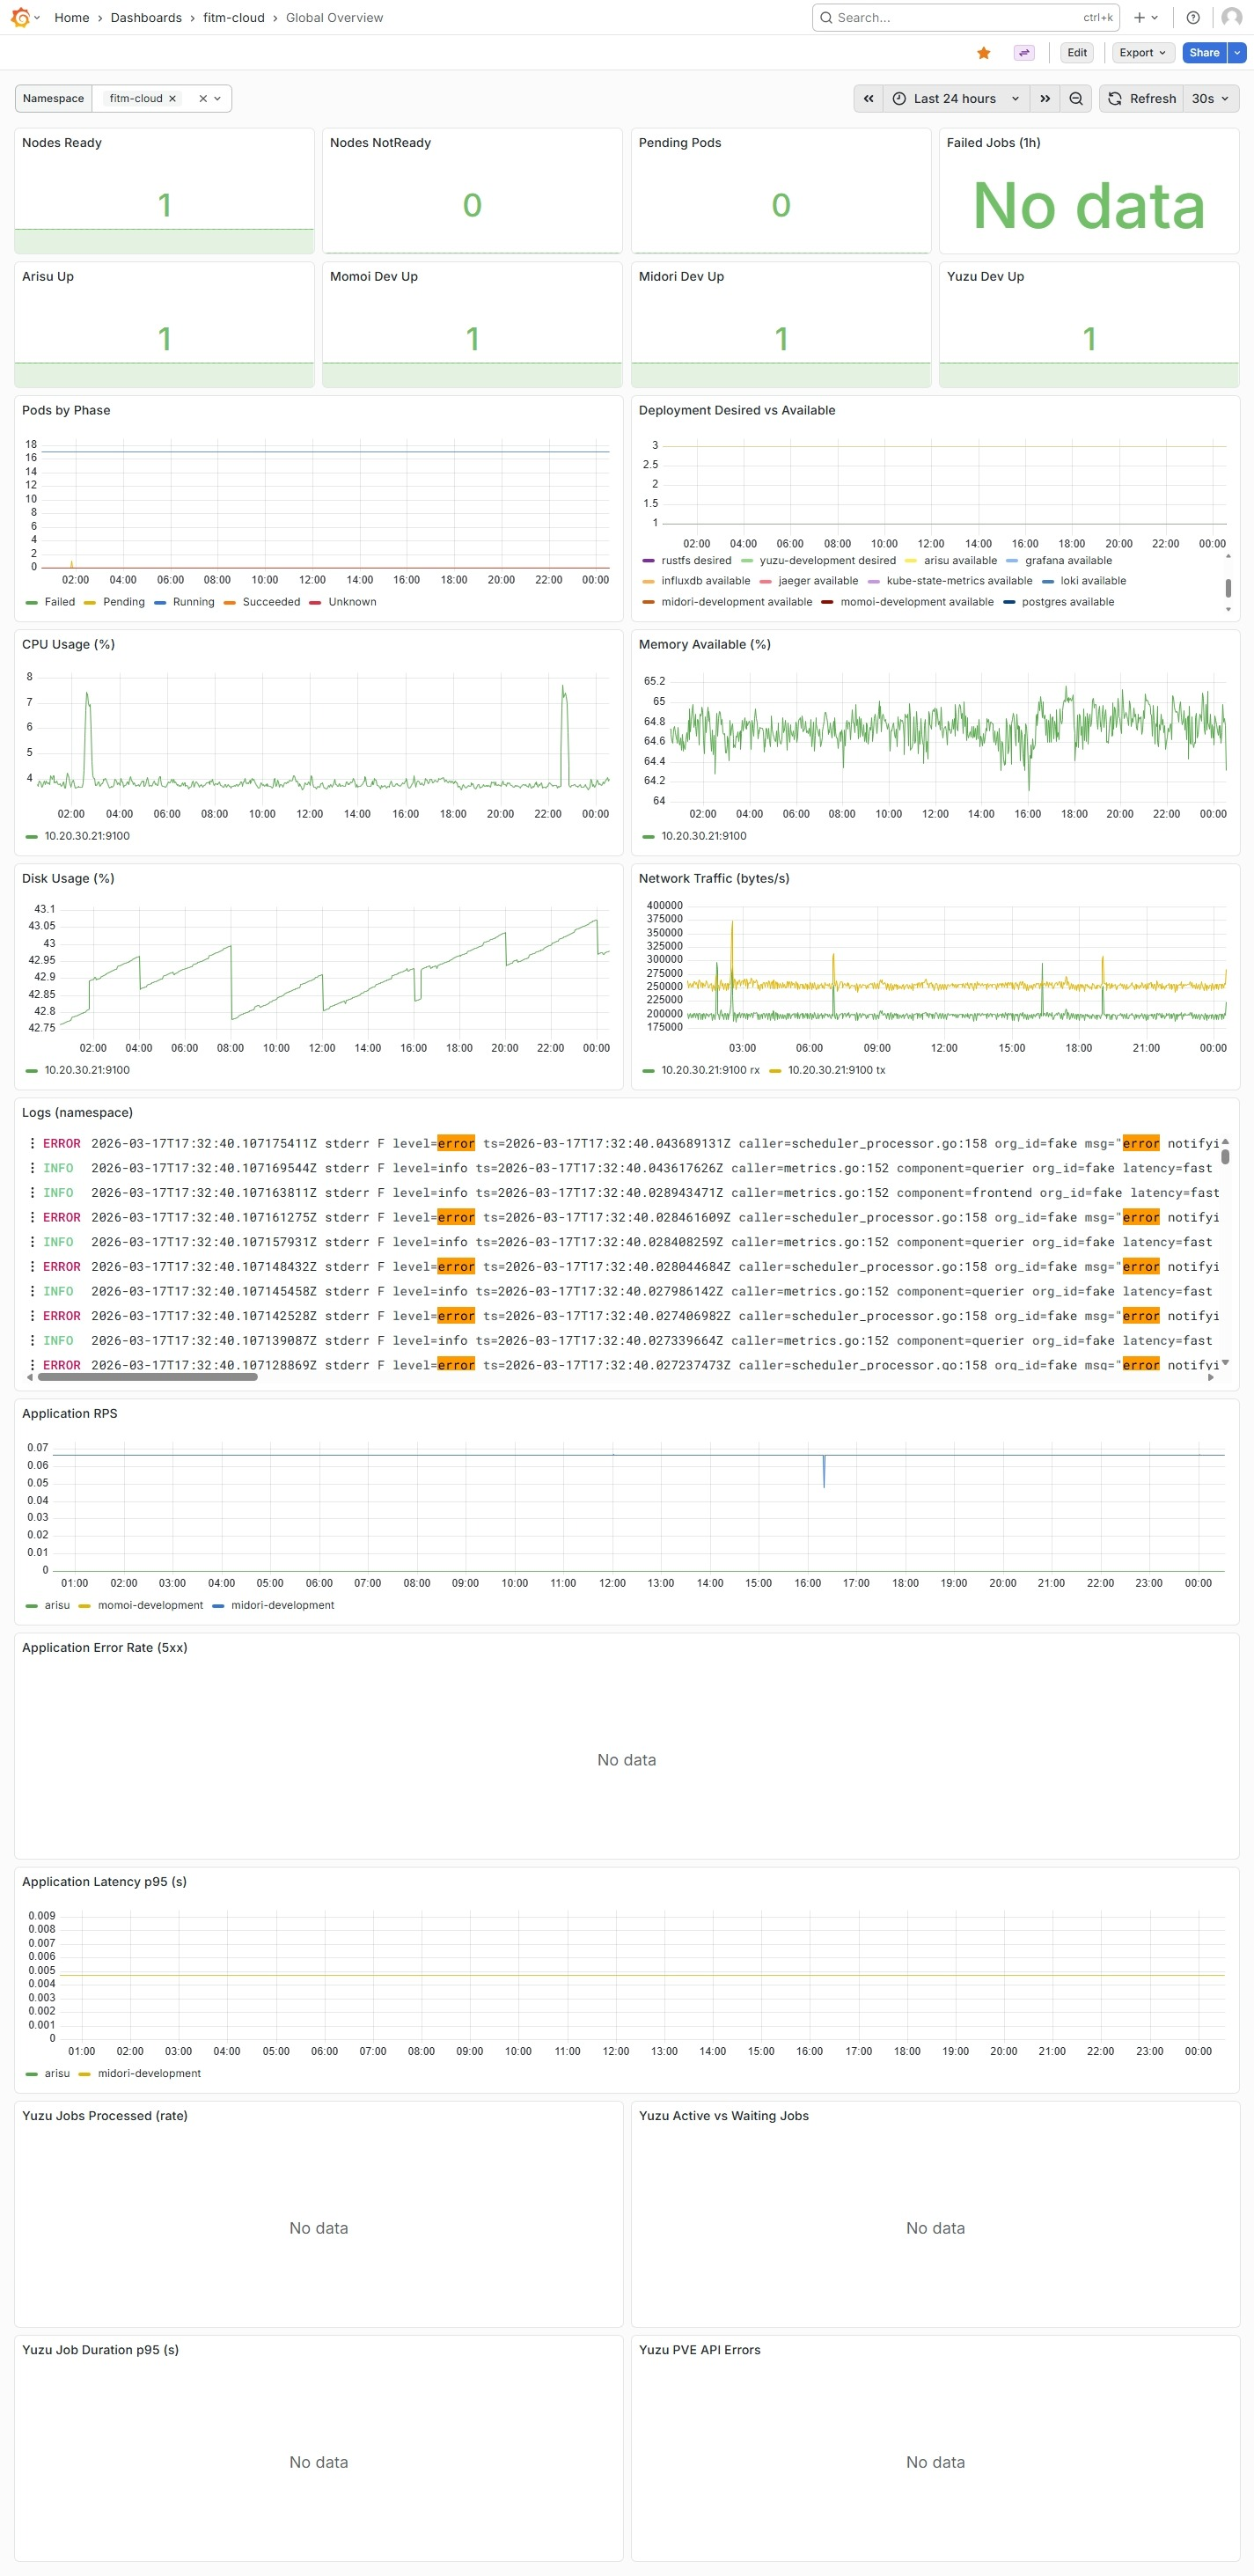
\includegraphics[width=1.0\textwidth]{Image/monitoring_dashboard.jpeg}
}
\caption{\fontSixTeen{ตัวอย่างผลการติดตามสถานะระบบบน Grafana Dashboard}}
\label{fig4:MonitoringDashboard}
\end{figure}

\subsection{ผลการติดตามแบบ Distributed Tracing ด้วย Jaeger}
\hspace*{1.3em}
Jaeger ถูกนำมาใช้เพื่อ trace การประมวลผลคำขอในเส้นทางที่เกี่ยวข้องกับ Midori และ Momoi ซึ่งช่วยในการระบุคอขวดและวิเคราะห์ latency ระหว่าง frontend และ API ได้อย่างมีประสิทธิภาพ สำหรับกระบวนการสร้างเครื่องเสมือนที่ต่อเนื่องไปยัง Redis Queue และ Yuzu นั้น ปัจจุบันการติดตามฝั่ง worker ยังพึ่งพา metrics และ logs มากกว่าการ trace แบบ end-to-end เต็มรูปแบบ ดังนั้นการวิเคราะห์ความล่าช้าในช่วงปฏิบัติการบน Proxmox VE จะอาศัยข้อมูลจาก queue metrics, worker logs และสถานะงานร่วมกัน

\hspace*{1.3em}
ภาพที่ \ref{fig4:MonitoringTrace} แสดงตัวอย่าง trace ที่รวบรวม span ของการประมวลผลคำขอในแต่ละชั้นบริการ ทำให้สามารถตรวจสอบขั้นตอนที่ใช้เวลามากผิดปกติและช่วยวิเคราะห์สาเหตุของความล่าช้าได้อย่างเป็นระบบ

\begin{figure}[H]
\centering
\adjustbox{frame, width=1.0\textwidth}{
    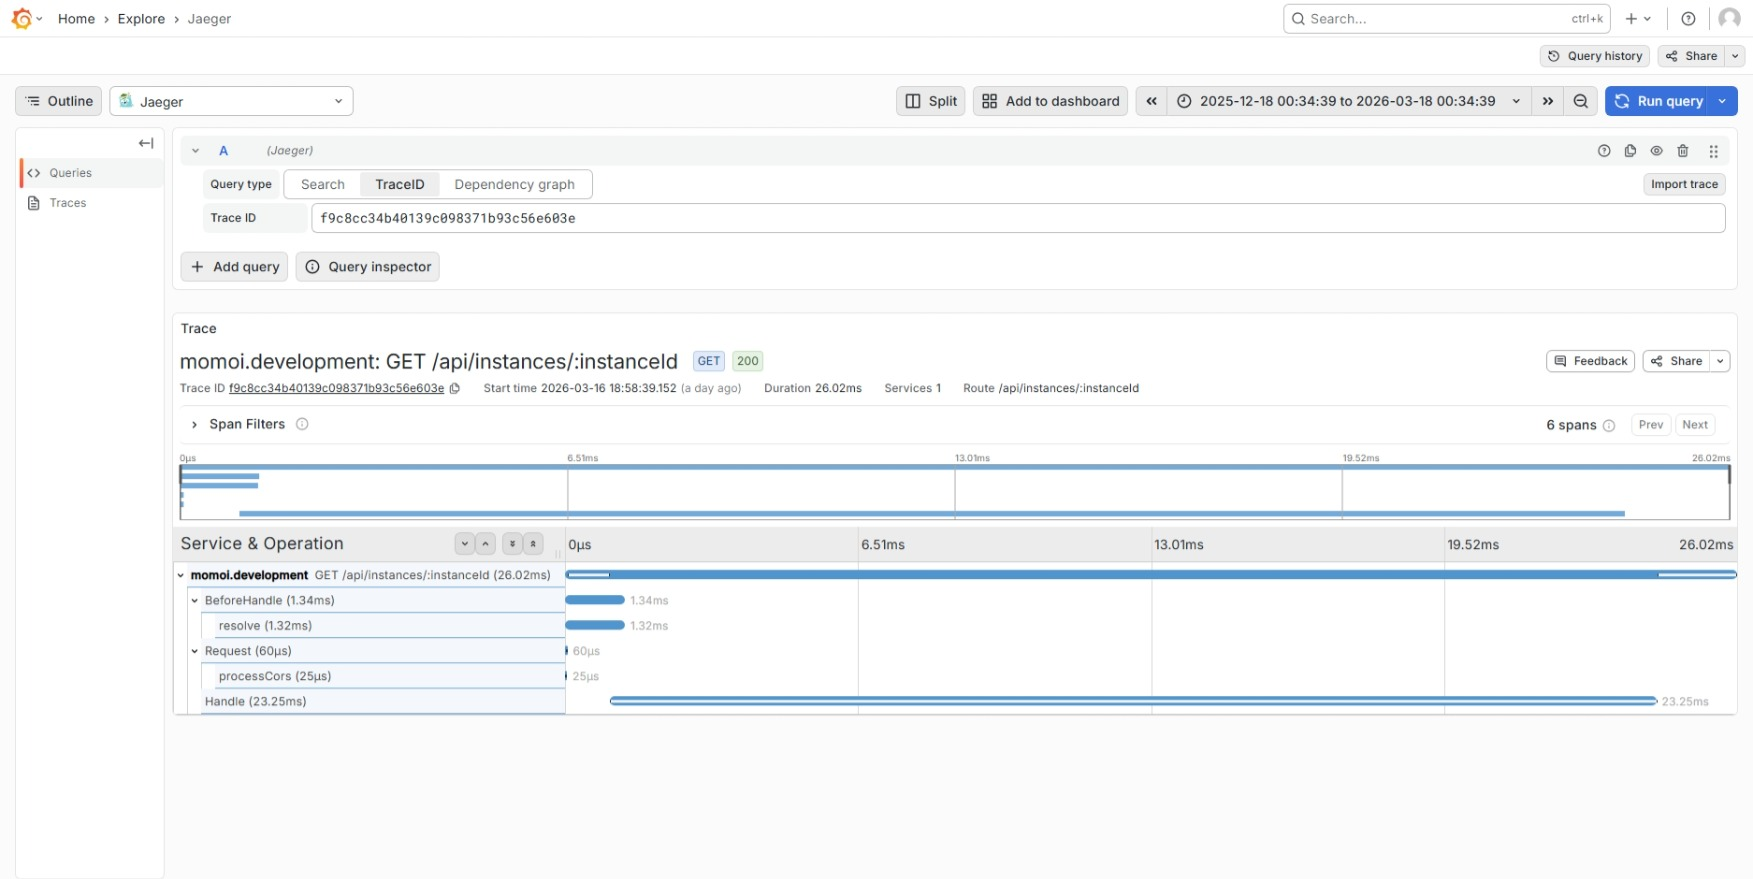
\includegraphics[width=1.0\textwidth]{Image/monitoring_dashboard_trace.jpeg}
}
\caption{\fontSixTeen{ตัวอย่างผลการติดตามเส้นทางคำขอ (Trace) บน Jaeger}}
\label{fig4:MonitoringTrace}
\end{figure}

\section{ผลการทดสอบประสิทธิภาพระบบ}
\label{sec:system-perf}
\hspace*{1.3em}
ส่วนนี้สรุปผลการทดสอบประสิทธิภาพของบริการหลักในระบบ โดยแบ่งตามบริการย่อย เพื่อให้เห็นภาพรวมและเปรียบเทียบสมรรถนะของแต่ละบริการได้อย่างชัดเจน

\subsection{ผลการทดสอบประสิทธิภาพส่วนติดต่อผู้ใช้ (Midori)}
\label{sec:midori-perf}
\hspace*{1.3em}
ทำการทดสอบสมรรถนะของ \textbf{Midori} (Frontend/Next.js) โดยมีเป้าหมายการทดสอบคือ \url{https://dev.fitm.cloud} ระยะเวลารวม 30 วินาที และระดับความขนานต่อเส้นทาง (Path-Level Parallelism) 100 พร้อมทั้งบันทึกรายละเอียดคำขอรายครั้งลงในไฟล์ log เพื่อใช้วิเคราะห์ความสม่ำเสมอของเวลาตอบสนองและพฤติกรรมในช่วง tail latency

\hspace*{1.3em}
ภาพรวมของการทดสอบสะท้อนปริมาณคำขอรวม 3{,}506 คำขอ อัตราความสำเร็จ 96.55\% และอัตราการส่งผ่านโดยเฉลี่ย 109.67 RPS ดังตารางที่ \ref{tab:midori-summary}

\begin{table}[htbp]
    \centering
    \caption{\fontSixTeen{สรุปผลภาพรวมการทดสอบ Midori}}
    \fontSixTeen
    \label{tab:midori-summary}
    \adjustbox{max width=\textwidth}{
        \begin{tabular}{@{}lrrrrr@{}}
            \hline
            เวลาเริ่ม & ระยะเวลา (s) & Requests & สำเร็จ & ล้มเหลว & Throughput (RPS) \\
            \hline
            2026-03-12 02:08:19Z & 30 & 3{,}506 & 3{,}385 & 121 & 109.67 \\
            \hline
        \end{tabular}
    }
\end{table}

\hspace*{1.3em}
การทดสอบครอบคลุมเส้นทางหลัก ได้แก่ หน้าแรกและหน้าลงชื่อเข้าใช้ ซึ่งเป็นเส้นทางสำคัญของส่วนติดต่อผู้ใช้ สถิติหลักสรุปในตารางที่ \ref{tab:midori-paths}

\begin{table}[htbp]
    \centering
    \caption{\fontSixTeen{ผลการทดสอบรายเส้นทาง (Midori)}}
    \label{tab:midori-paths}
    \fontSixTeen
    \adjustbox{max width=\textwidth}{
        \begin{tabular}{@{}lrrrrrrrr@{}}
            \hline
            เส้นทาง & Requests & สำเร็จ & ล้มเหลว & RPS & p50 (ms) & p95 (ms) & p99 (ms) & max (ms) \\
            \hline
            / & 1{,}730 & 1{,}670 & 60 & 54.12 & 699.18 & 12{,}858.73 & 15{,}008.66 & 15{,}015.25 \\
            /login & 1{,}776 & 1{,}715 & 61 & 55.81 & 705.81 & 11{,}971.10 & 15{,}006.54 & 15{,}016.48 \\
            \hline
        \end{tabular}
    }
\end{table}

% \newpage
\hspace*{1.3em}
\textbf{ข้อสังเกตและข้อเสนอแนะเบื้องต้น}
\begin{mycustomitem}
    \item ผลการทดสอบแสดงให้เห็นว่า Midori ยังให้บริการได้ต่อเนื่องภายใต้โหลด 100 concurrent users ต่อเส้นทาง แต่มี tail latency สูงมาก โดยค่า p95 และ p99 ของทั้งสองหน้าแตะระดับ 11.9--15.0 วินาที และมีคำขอล้มเหลวรวม 121 ครั้ง
    \item จากไฟล์บันทึกรายคำขอ พบว่าคำขอส่วนหนึ่งในช่วงต้นและช่วงกลางของการทดสอบตอบกลับได้ในช่วงประมาณ 80--900 ms แต่มีอีกกลุ่มหนึ่งชนเพดาน timeout ของสคริปต์ที่ประมาณ 15 วินาที สอดคล้องกับค่า max latency ที่สูงมากในผลสรุป
    \item หน้าแรกและหน้าลงชื่อเข้าใช้มีสมรรถนะใกล้เคียงกัน โดย p50 อยู่ราว 700 ms แสดงว่าคอขวดน่าจะอยู่ที่ชั้นการ render หรือการเรียกทรัพยากรร่วมมากกว่าจะเป็นเพียงหน้าใดหน้าหนึ่งโดยเฉพาะ
    \item หากต้องการปรับปรุงผลลัพธ์ ควรตรวจสอบการทำ caching ของ Next.js, การโหลด asset และ data fetching ที่เกิดในฝั่ง server, รวมถึงการตั้งค่า reverse proxy และ connection reuse ระหว่าง Midori กับบริการปลายทาง เพื่อกด tail latency และลดจำนวนคำขอที่ timeout
\end{mycustomitem}

\subsection{ผลการทดสอบประสิทธิภาพบริการ API (Momoi)}
\label{sec:momoi-perf}
\hspace*{1.3em}
เพื่อประเมินสมรรถนะของบริการ \textbf{Momoi} (API Service) ได้ดำเนินการทดสอบภาระงานด้วยการยิงคำขอพร้อมกันต่อเส้นทาง (per-path concurrency) โดยมีเป้าหมายการทดสอบคือ \url{https://dev.fitm.cloud} ที่ระยะเวลารวม 30 วินาที และระดับความขนานต่อเส้นทาง 100 พร้อมบันทึกผลรายคำขอทุกครั้งลงไฟล์ log เพื่อใช้วิเคราะห์เสถียรภาพของ API ภายใต้โหลดจริง

\hspace*{1.3em}
ภาพรวมของการทดสอบสะท้อนปริมาณคำขอรวม 7{,}216 คำขอ อัตราความสำเร็จ 100\% และอัตราการส่งผ่านโดยเฉลี่ย 234.87 RPS ดังตารางที่ \ref{tab:momoi-summary}

\begin{table}[htbp]
    \centering
    \caption{\fontSixTeen{สรุปผลภาพรวมการทดสอบ Momoi API}}
    \fontSixTeen
    \label{tab:momoi-summary}
    \begin{tabular}{lrrrrr}
        \hline
    เวลาเริ่ม & ระยะเวลา (s) & Requests & สำเร็จ & ล้มเหลว & Throughput (RPS) \\
        \hline
    2026-03-12 02:12:46Z & 30 & 7{,}216 & 7{,}216 & 0 & 234.87 \\
        \hline
    \end{tabular}
\end{table}

\hspace*{1.3em}
จากข้อมูลสรุป ครั้งนี้คำขอทั้งหมดสำเร็จ (ค่า ok=\,7{,}216) สะท้อนว่าเส้นทาง API ที่เลือกทดสอบยังคงทำงานได้ถูกต้องภายใต้เงื่อนไขการทดสอบดังกล่าวตามข้อมูลในตารางที่ \ref{tab:momoi-paths}

\begin{table}[htbp]
    \centering
    \caption{\fontSixTeen{ผลการทดสอบรายเส้นทาง (Momoi API)}}
    \fontSixTeen
    \label{tab:momoi-paths}
    \adjustbox{max width=\textwidth}{
        \begin{tabular}{@{}lrrrrrrrr@{}}
            \hline
            เส้นทาง & Requests & สำเร็จ & ล้มเหลว & RPS & p50 (ms) & p95 (ms) & p99 (ms) & max (ms) \\
            \hline
            /api/openapi/json & 4{,}228 & 4{,}228 & 0 & 137.73 & 566.46 & 987.09 & 1{,}479.75 & 1{,}688.93 \\
            /api/academic/semesters/current & 2{,}988 & 2{,}988 & 0 & 97.25 & 987.90 & 1{,}308.27 & 1{,}740.05 & 2{,}736.64 \\
            \hline
        \end{tabular}
    }
\end{table}

\hspace*{1.3em}
\textbf{ข้อสังเกตและข้อเสนอแนะเบื้องต้น}
\begin{mycustomitem}
    \item Momoi มีเสถียรภาพสูงภายใต้โหลด 100 concurrent users ต่อเส้นทาง โดยไม่มีคำขอล้มเหลวเลย และยังคงรักษา throughput รวมได้ประมาณ 234.87 RPS บนโดเมนพัฒนา
    \item เส้นทาง \textit{/api/openapi/json} มี throughput สูงกว่าเส้นทาง \textit{/api/academic/semesters/current} แม้ว่าจะมีขนาดข้อมูลตอบกลับสูงมาก โดยจาก log รายคำขอพบว่าขนาดตอบกลับของ OpenAPI อยู่ที่ประมาณ 218{,}193 ไบต์ต่อคำขอ และสร้างปริมาณข้อมูลรวมมากกว่า 880 MB ตลอดการทดสอบ
    \item เส้นทาง \textit{/api/academic/semesters/current} มี payload ขนาดเล็กมากประมาณ 195 ไบต์ต่อคำขอ แต่กลับมี p50 สูงกว่าเส้นทาง OpenAPI อย่างชัดเจน สะท้อนว่าคอขวดหลักน่าจะเกิดจากการประมวลผลใน handler หรือการเข้าถึงข้อมูล backend มากกว่าขนาด response เพียงอย่างเดียว
    \item จาก log รายคำขอในช่วงต้นของการทดสอบพบว่าค่า latency ของ \textit{/api/openapi/json} ส่วนใหญ่อยู่ประมาณ 680--1{,}160 ms ขณะที่ \textit{/api/academic/semesters/current} กระจุกอยู่ราว 1{,}224--1{,}740 ms ซึ่งสอดคล้องกับค่า percentile ในผลสรุป และบ่งชี้ว่าระบบมีความสม่ำเสมอแม้อยู่ภายใต้โหลดต่อเนื่อง
    \item หากต้องการลด latency ของเส้นทางเชิงธุรกิจ ควรตรวจสอบ query path ของ endpoint ภาคการศึกษาปัจจุบัน การใช้ cache สำหรับข้อมูลที่เปลี่ยนไม่บ่อย และการแยกเส้นทางเอกสาร OpenAPI ออกจาก traffic ใช้งานจริงเมื่อทำการทดสอบเชิงเปรียบเทียบในอนาคต
\end{mycustomitem}

\subsection{ผลการทดสอบประสิทธิภาพบริการจัดการเครื่องเสมือน (Yuzu)}
\label{sec:yuzu-perf}
\hspace*{1.3em}
เพื่อประเมินสมรรถนะของบริการ \textbf{Yuzu} ได้ทำการทดสอบการโคลนเครื่องเสมือน (VM Clone) เปรียบเทียบระหว่างวิธี \textit{Linked Clone} และ \textit{Full Clone} โดยใช้แม่แบบ VM เดียวกันและกระจายงานไปยังโหนดปลายทางหลายเครื่อง

\hspace*{1.3em}
ในการตีความผลการทดสอบส่วนนี้ ควรระบุขอบเขตของการวัดเวลาให้ชัดเจนว่าเวลาที่รายงานครอบคลุมเฉพาะช่วงการสร้างหรือโคลนเครื่องเสมือนจนกระทั่งงานฝั่งโครงสร้างพื้นฐานเสร็จสิ้นในระดับที่ระบบสามารถส่งต่อไปยังขั้นตอนถัดไปได้เท่านั้น แต่ยัง \textbf{ไม่ได้รวม} เวลาของกระบวนการ \textit{cloud-init} หลังบูตเครื่อง เช่น การตั้งค่าเริ่มต้น การอัปเดตแพ็กเกจ และการอัปเกรดแพ็กเกจภายใน guest OS ซึ่งจากการสังเกตการใช้งานจริงอาจใช้เวลาเพิ่มได้อีกราว 3 นาที ก่อนที่เครื่องจะอยู่ในสภาพพร้อมใช้งานเต็มรูปแบบ

\hspace*{1.3em}
ภาพรวมการทดสอบประกอบด้วยทั้งหมด 20 เคส โดยเป็น Linked Clone 10 เคส และ Full Clone 10 เคส สถานะสำเร็จ/ล้มเหลวและเวลาที่ใช้สรุปได้ดังตารางที่ \ref{tab:yuzu-clone-summary} และข้อสังเกตที่ตามมา

\begin{table}[htbp]
    \centering
    \caption{\fontSixTeen{สรุปผลการทดสอบการโคลน VM: Linked vs Full}}
    \fontSixTeen
    \label{tab:yuzu-clone-summary}
    \begin{tabular}{lrrrrr}
        \hline
        วิธีโคลน & จำนวนนับ & สำเร็จ & ล้มเหลว & เวลาเฉลี่ย (ms) & ช่วงเวลา (min/max ms) \\
        \hline
        Linked & 10 & 10 & 0 & 5{,}931.49 & 1{,}492.12 / 10{,}423.62 \\
        Full & 10 & 3 & 7 & 172{,}493.80\,\footnotemark & 167{,}395.68 / 175{,}525.81 \\
        \hline
    \end{tabular}
\end{table}
\footnotetext{เวลาเฉลี่ยของ Full Clone คำนวณจากเคสที่สำเร็จ (3 เคส) ตามข้อมูลในไฟล์ผลการทดสอบ}

\hspace*{1.3em}
เมื่อเปรียบเทียบเวลาเฉลี่ย วิธี \textbf{Linked Clone} เร็วกว่าวิธี \textbf{Full Clone} โดยเฉลี่ยประมาณ 166{,}562.31 ms หรือคิดเป็นร้อยละ 96.56 ของเวลาที่ลดลง ซึ่งสอดคล้องกับสถาปัตยกรรมการใช้งาน \textit{copy-on-write} ของ Linked Clone ที่ไม่คัดลอกดิสก์เต็มทั้งลูกในขั้นตอนเริ่มต้น

\hspace*{1.3em}
อย่างไรก็ตาม หากพิจารณาในมุมของ \textit{time-to-usable-instance} หรือเวลาตั้งแต่เริ่ม provision จนผู้ใช้สามารถเข้าใช้งานเครื่องได้จริง ระยะเวลาที่รับรู้ได้จริงจะยาวกว่าค่าที่แสดงในตาราง เนื่องจากยังต้องรวมช่วง boot และขั้นตอน cloud-init ภายในเครื่อง โดยเฉพาะงาน \textit{packages update/upgrade} ที่อาจเพิ่มเวลาได้อีกราว 180 วินาที ทำให้แม้ Linked Clone จะเสร็จในระดับโครงสร้างพื้นฐานภายในไม่กี่วินาที แต่เวลาพร้อมใช้งานจริงของเครื่องอาจอยู่ในระดับประมาณ 3--4 นาที ขณะที่ Full Clone อาจสูงกว่านั้นอย่างมีนัยสำคัญ

\hspace*{1.3em}
\textbf{ข้อสังเกตและการวิเคราะห์}
\begin{mycustomitem}
    \item อัตราความสำเร็จ: Linked Clone สําเร็จ 100\% (10/10) ในขณะที่ Full Clone สําเร็จ 30\% (3/10)
    \item สาเหตุความล้มเหลวของ Full Clone: พบข้อความผิดพลาด เช่น "cfs-lock 'storage-rbd' error: got lock request timeout" และ "failed with exit status: WARNINGS: 1" ซึ่งบ่งชี้ถึงปัญหาการล็อกทรัพยากรของระบบจัดเก็บข้อมูลแบบ RBD/คลัสเตอร์ หรือข้อจํากัดด้านโควตา/นโยบายของสตอเรจ
    \item ความแปรปรวนของเวลา: เคส Linked Clone มีช่วงเวลาตั้งแต่ ~1.49 วินาที ถึง ~10.42 วินาที ขึ้นอยู่กับโหนดปลายทางและภาระงาน ณ ขณะนั้น ขณะที่ Full Clone ที่สําเร็จใช้เวลาประมาณ 167 – 175 วินาที (2.8 – 2.9 นาที) ต่อเคส
    \item ขอบเขตของเวลาในผลทดสอบ: ตัวเลขในตารางยังไม่รวมระยะเวลา cloud-init หลังบูตเครื่อง ดังนั้นเวลาพร้อมใช้งานจริงของเครื่องเสมือนจะสูงกว่าค่าที่รายงาน โดยเฉพาะกรณีที่ guest OS มีการสั่ง \textit{update} และ \textit{upgrade} แพ็กเกจระหว่างเริ่มต้นระบบ
    \item ผลกระทบต่อการออกแบบระบบ: สำหรับงานสอนที่ต้องสร้าง VM จำนวนนักศึกษามากในเวลาจำกัด Linked Clone ให้เวลาโปรวิชันรวดเร็วอย่างมีนัยสําคัญ และลดความเสี่ยงจากคอขวดด้าน IO ของสตอเรจส่วนกลาง
\end{mycustomitem}

% \newpage
\hspace*{1.3em}
\textbf{ข้อเสนอแนะเชิงปฏิบัติ}
\begin{mycustomitem}
    \item ใช้ Linked Clone เป็นค่าเริ่มต้นในการโปรวิชัน VM จํานวนมาก โดยเฉพาะกรณีแล็บการสอนหรือกิจกรรมที่เน้นความรวดเร็วในการเริ่มใช้งาน
    \item หากต้องการวัดประสบการณ์ใช้งานจริงของผู้ใช้ ควรเพิ่มตัวชี้วัดจาก \textit{clone completed} ไปเป็น \textit{instance ready after cloud-init} เช่น รอจน cloud-init เสร็จและบริการพื้นฐานตอบสนองได้ เพื่อสะท้อนเวลาพร้อมใช้งานจริงของเครื่อง
    \item สําหรับ Full Clone ให้พิจารณาโหมดคิวงาน/การจัดคิวแบบจํากัดพร้อมกัน (throttling) และปรับ \textit{timeout} ของการล็อกสตอเรจ เพื่อหลีกเลี่ยง \textit{cfs-lock} timeout
    \item ตรวจสอบคอนฟิกสตอเรจ RBD/คลัสเตอร์ (เช่น พารามิเตอร์ Ceph/RBD, คิวงานบน Proxmox VE, และเครือข่ายสตอเรจ) เพื่อบรรเทาข้อความผิดพลาดประเภท WARNINGS และเพิ่มอัตราสำเร็จของ Full Clone
    \item พิจารณาปรับภาพแม่แบบให้ลดงานที่ต้องทำในช่วง cloud-init เช่น เตรียมแพ็กเกจพื้นฐานไว้ล่วงหน้า หรือแยกงาน \textit{update/upgrade} ที่ใช้เวลานานออกจากเส้นทาง provision หลัก เพื่อลดเวลารอจริงของผู้ใช้
    \item เฝ้าติดตามตัวชี้วัด IO/ล็อกของสตอเรจระหว่างช่วงพีก และทดสอบซ้ำหลังปรับแต่ง เพื่อยืนยันการปรับปรุง
\end{mycustomitem}
